%% LaTeX2e class for student theses
%% sections/evaluation.tex
%% 
%% Karlsruhe Institute of Technology
%% Institute for Program Structures and Data Organization
%% Chair for Software Design and Quality (SDQ)
%%
%% Dr.-Ing. Erik Burger
%% burger@kit.edu
%%
%% Version 1.3.6, 2022-09-28

\chapter{Evaluation}
\label{ch:Evaluation}

In the following chapter we will evaluate the experiments we conducted. We start off by explaining our evaluation metrics, both for Continual Active Learning
and when applying Continual Active Learning to Model Stealing. Afterwards we will present the results of our experiments and discuss the findings.

\section{Evaluation Metrics}
\label{sec:Evaluation:Metrics}
% Describe that we used agreement for model stealing (and on which dataset) and 
% validation accuracy for the model stealing experiments. and hyperparameters

\subsection{Metrics for Continual Active Learning}
\label{sec:Evaluation:Metrics:CAL}
When choosing a metric to evaluate Continual Active Learning, we need to remember the motivation of the approach. We proposed the Continual Active Learning approach
mainly to reduce the mainly to mitigate the overhead of pure Active Learning compared to the classic training loop. Therefore, it is desirable to incorporate a metric
which measures this goal. In our case, this is the overall execution time. However, execution time is not the only metric we want to use to evaluate the approach. Since 
the second goal of the Continual Learning approach is to improve model performance, we will also evaluate the experiments based on this. What a makes a machine learning 
model performant has been discussed vividly in the literature. In our case, we will use the validation accuracy as a metric to evaluate the performance of the model. It is
important to consider \textit{both} runtime and validation accuracy when evaluating the experiments. A model with low runtime and low validation accuracy is not desirable,
but neither is a model with high runtime and high validation accuracy. Since we are trying to improve Active Learning by introducing Continual Learning into the pool-based 
Active Learning process, we aim to outperform the classic pool-based Active Learning approach. More precisely, we want to reduce the runtime and increase the validation
accuracy. The success of our Continual Active Learning approach will be evaluated against the classic pool-based Active Learning approach based on the runtime improvement
and the accuracy improvement. 


\subsection{Metrics for Continual Active Learning for Model Stealing}
\label{sec:Evaluation:Metrics:CALMS}
As presented in section \ref{sec:ModelStealing:Attacks}, Model Stealing Attacks can be performed for a variety of reasons. As we build our framework on ActiveThief, we also
adopt the metrics used in the original paper. The ActiveThief framework aims purely at stealing the functionality of the model, i.e. approximation the model's relationship
between input and output best, and so does ours. Therefore, we will use the same evaluation metric, which in our case is the agreement between substitute and target model,
computed on the validation split of the target model dataset. The baseline which we compare our results against is the ActiveThief framework. We will therefore measure the 
success of using Continual Active Learning for Model Stealing by comparing the model agreement of our approach to the model agreement of the ActiveThief framework.

\section{Results}
\label{sec:Evaluation:Results}
In this section we will present the results of our experiments. As mentioned before, our experiments are split into two parts. The first part is the evaluation of our novel
Continual Active Learning Approach and the second part is evaluating the performance our the Continual Active Learning approach when applied to Model Stealing. In each of these
respective subsections we will first describe the experiments schedule for each part and then present the results of the experiments.

\subsection{Results for Continual Active Learning}
\label{sec:Evaluation:Results:CAL}
In this subsection we will first present the results of running all combinations of the Active Learning strategies BALD,Badge,CoreSet,LC and Random with the Continual Learning strategies
Naive, EWC, MAS, Alasso and IMM. Afterwards, we will analyze the behavior of a hybrid approach between Active Learning and Continual Active Learning, where we first run a few cycles with
pure Active Learning before switching to Continual Active Learning. We further analyze the performance of different strategies to initialize the labeled pool. Next, we experiment with VAAL
and AGEM.

\subsubsection{AL and Cl combinations}
\label{sec:Evaluation:Results:CAL:ALCL}
To evaluate the combination of the Active Learning strategies BALD,Badge,Coreset,LC and Random with the Continual Learning strategies Naive, EWC, MAS, Alasso and IMM, we run each combination
using a batch size of 1000,2000 and 4000. We use the CIFAR-10 dataset and the Neural Network Architecture Resnet18 for these experiments. We present the validation accuracy with increasing
size of the labeled pool as well as the overall runtime of each experiment. \par
In figure \ref{fig:Evaluation:Results:CAL:Random1000} we present the results of running the Active Learning strategy Random with the Continual Learning strategies Naive, EWC, MAS, Alasso and IMM
as well as the baseline of running pure Active Learning. We use a batch size of 1000 for these experiments. In terms of runtime, all strategies are significantly faster than the classic Active
Learning approach. MAS, IMM, EWC and Naive all are approximately 50 times as fast as the classic Active Learning approach. Alasso is slightly slower than the other Continual Learning strategies,
but still about 25 times faster than the baseline. However, there is a notable gap in validation accuracy between Active Learning and all Continual Active Learning strategies. IMM is the only
Continual Learning strategy to outperform the Naive approach. EWC performs slightly worse Naive while MAS and Alasso perform significantly worse. While the validation accuracy of MAS increases only
slightly with an increasing size of the labeled pool, Alasso has an erratic validation curve which does not seem to stabilize until the end of the experiment. \par
\begin{figure}[h]
    \centering
    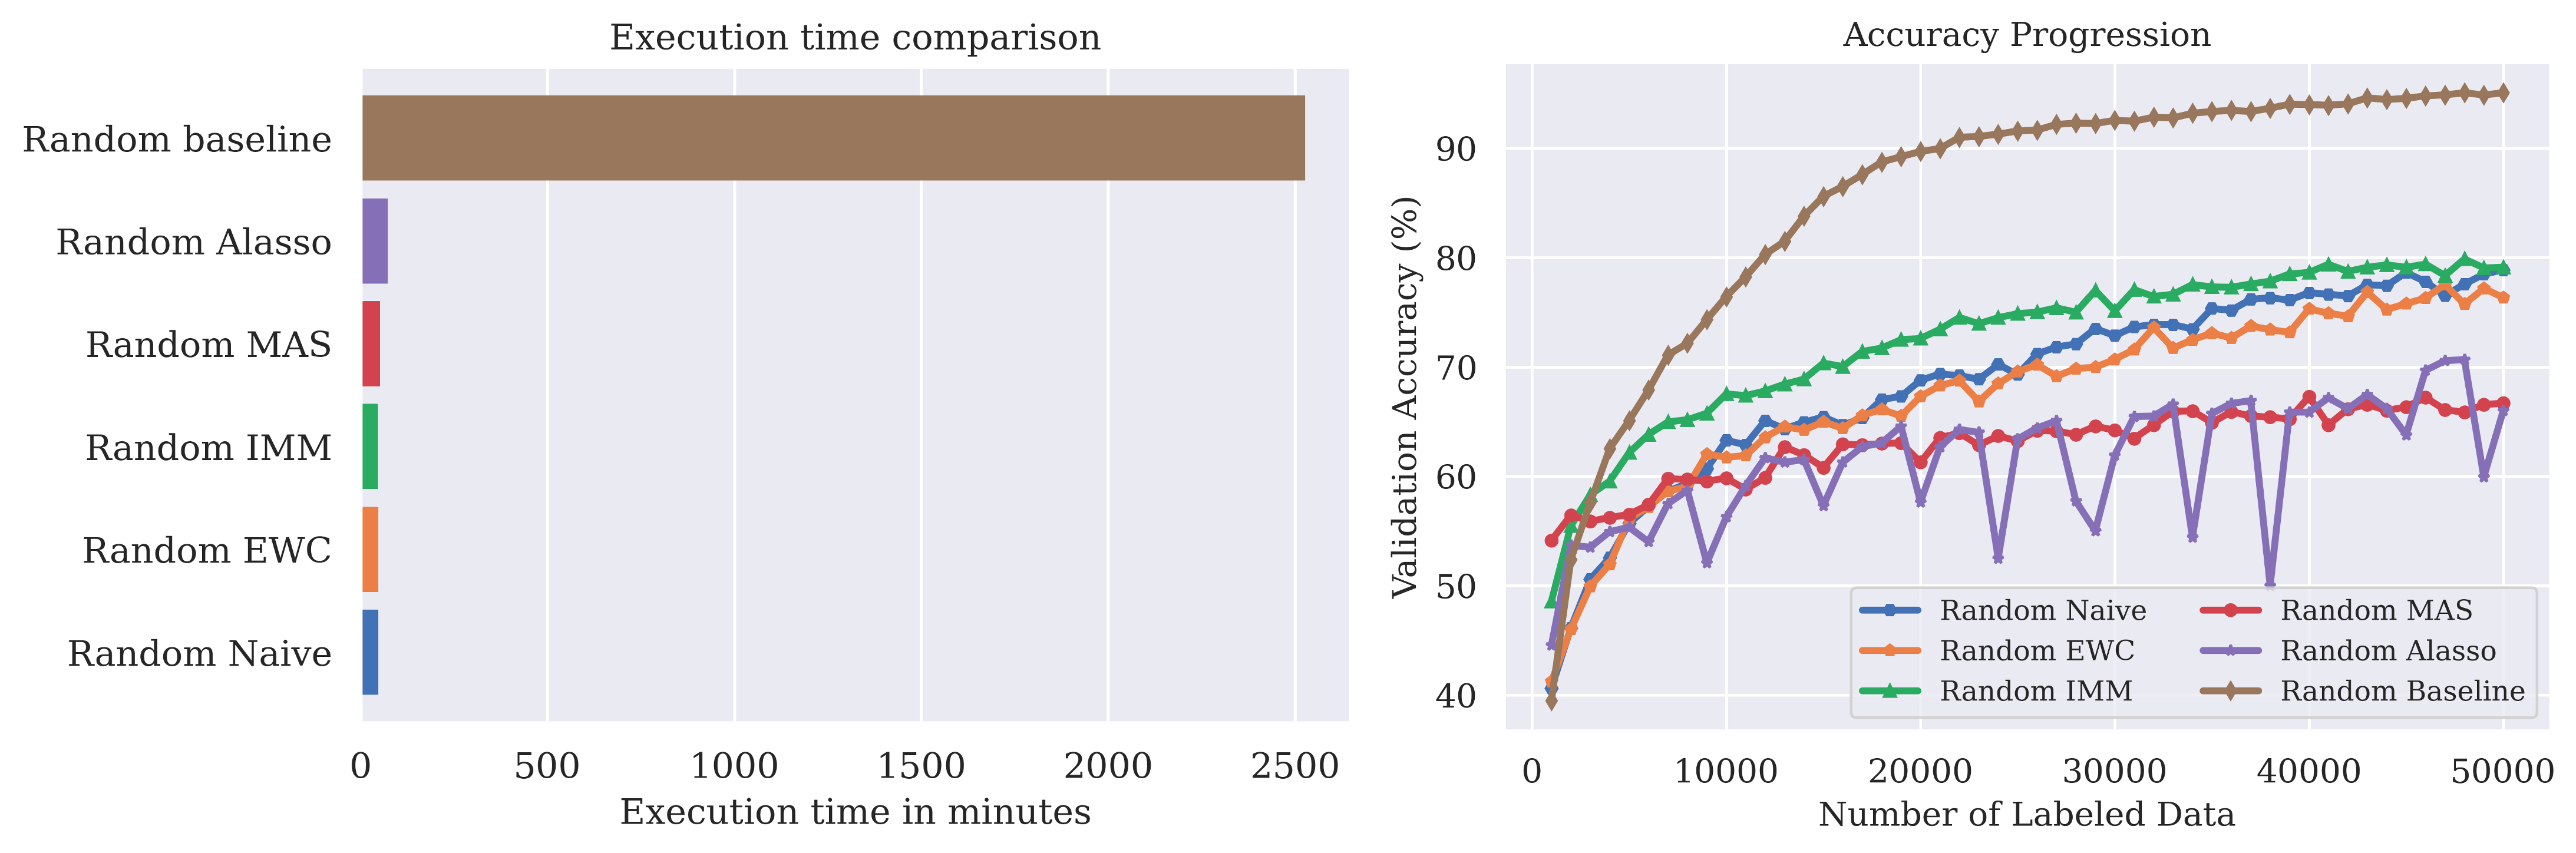
\includegraphics[width=\linewidth]{images/results_CAL/Random_CAL_1000b.png}
    \caption[Continual Active Learning Random 1000 batch size]{Comparison of execution time and validation accuracy of Continual Learning strategies used with the Active Learning strategy random.
    We use a batch size of 1000 for the experiments.}
    \label{fig:Evaluation:Results:CAL:Random1000}
\end{figure}

Next, we run the same experiment setup with the Active Learning strategy LC. Results can be found in figure \ref{fig:Evaluation:Results:CAL:LC1000}. Again, all Continual Learning strategies
are significantly outperform the baseline in terms of execution time. Alasso is the slowest Continual Learning strategy, albeit being roughly 25 times faster than the baseline. The remaining Continual
Learning strategies, IMM, MAS, CoreSet and EWC, are all about 50 times faster than the baseline. The gap in validation accuracy between Active Learning and all Continual Active Learning strategies
remains similar to the gap observed with Random. IMM and Naive perform similarly, outperforming the remaining Continual Learning strategies in the first half of the experiment. EWC picks up on their
performance in the after 25000 sampled data. MAS and Alasso fall behind in terms of performance, with Alasso experiencing significant accuracy drops. MAS' validation accuracy remain stable throughout
the whole experiment, catching up to the other Continual Learning strategies in the end. \par

\begin{figure} [h]
    \centering
    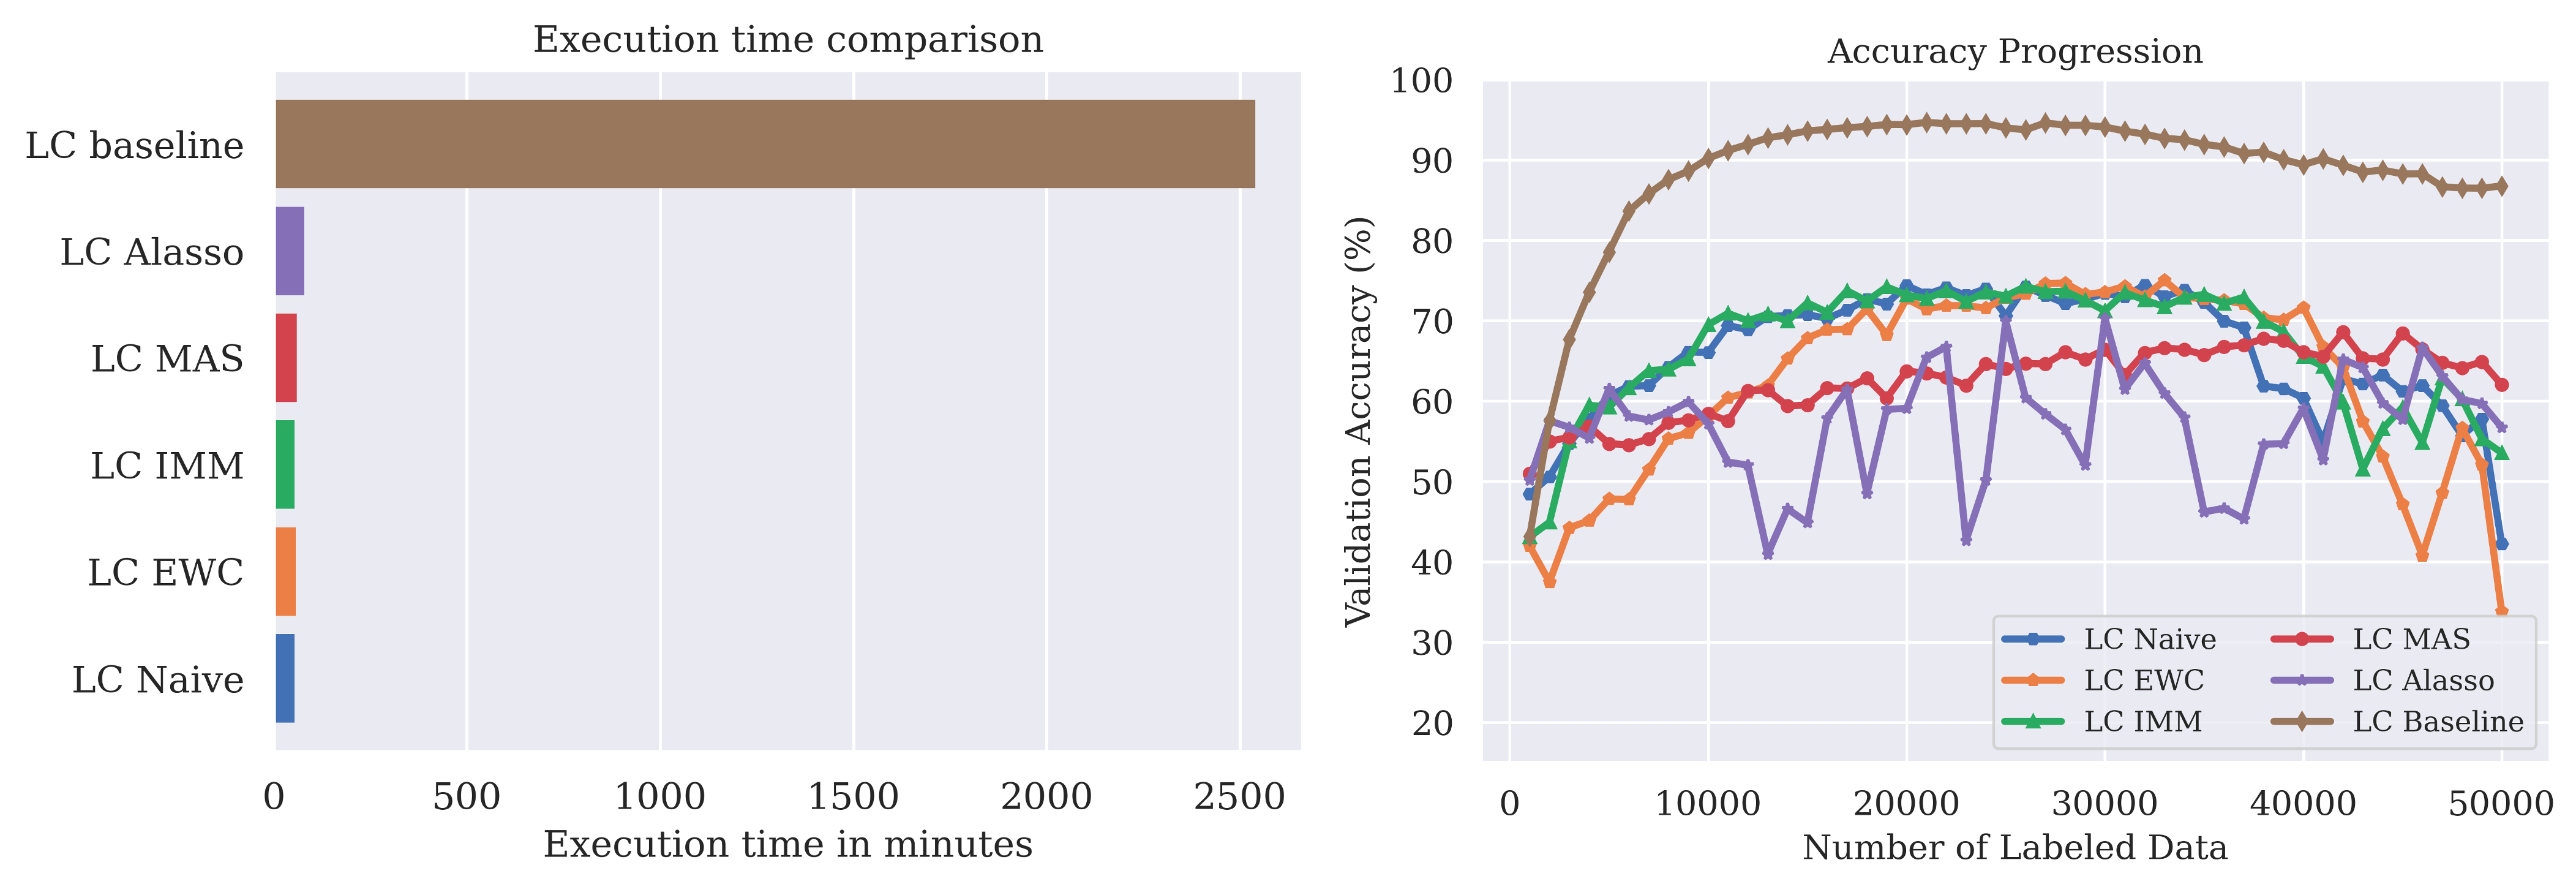
\includegraphics[width=\linewidth]{images/results_CAL/LC_CAL_1000b.png}
    \caption[Continual Active Learning LC 1000 batch size]{Comparison of execution time and validation accuracy of Continual Learning strategies used with the Active Learning strategy LC.
    We use a batch size of 1000 for the experiments.}
    \label{fig:Evaluation:Results:CAL:LC1000}
\end{figure}

BALD is the third Active Learning strategy we evaluate. Again, we use the same experiments setup as in the previous two experiments, changing only the Active Learning strategy but leaving every-
thing else as-is. The results of these experiments can be found in figure \ref{fig:Evaluation:Results:CAL:BALD1000}. In terms of runtime, the pattern established using LC and Random continues.
MAS, IMM, EWC and Naive are approximately 50 times as fast as the baseline, while Alasso is about 25 times as fast. Considering validation accuracy, all Continual Learning strategies perform significantly
worse than the baseline. Establishing a ranking between the Continual Learning strategies is difficult however, because they are all very erratic. Alasso stands out with the best and worst validation
accuracy, depending on the number of labeled samples. IMM, MAS, Naive and EWC all have similar validaiton accuracy curves, although they are less erratic than Alasso. \par

\begin{figure}[h]
    \centering
    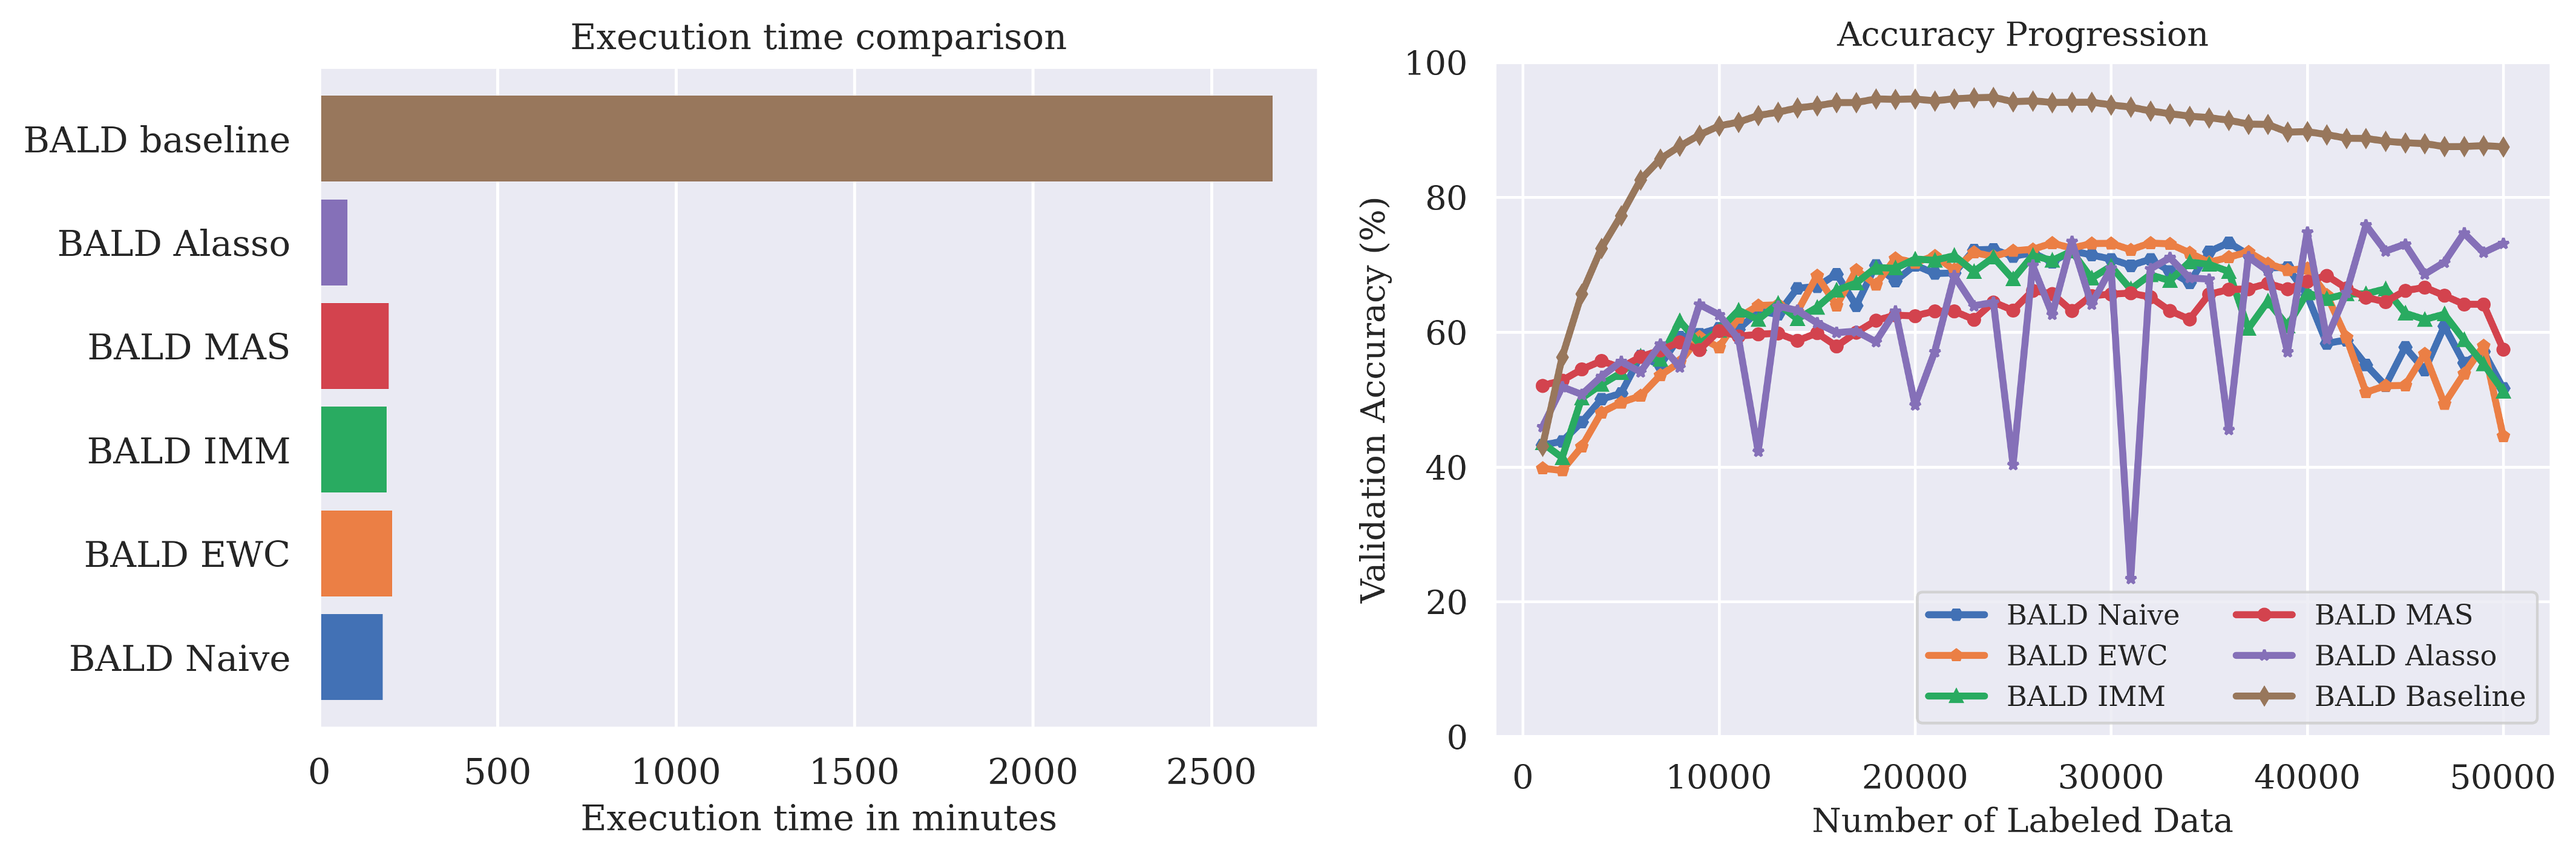
\includegraphics[width=\linewidth]{images/results_CAL/Bald_CAL_1000b.png}
    \caption[Continual Active Learning BALD 1000 batch size]{Comparison of execution time and validation accuracy of Continual Learning strategies used with the Active Learning strategy BALD.
    We use a batch size of 1000 for the experiments.}
    \label{fig:Evaluation:Results:CAL:BALD1000}
\end{figure}

After running our experiment with BALD, we re-run it using the Active Learning strategy CoreSet. We present the results in figure \ref{fig:Evaluation:Results:CAL:CoreSet1000}. The runtime of the 
Continual Learning strategies is again significantly lower than that of the baseline, however it is higher than in the previous experiments. Alasso is the slowest Continual Learning strategy, being
around 12 times as fast as the baseline. IMM, MAS, EWC and Naive have a similar execution time and are approximately 15 times as fast as Active Learning using CoreSet. Just as in the previous experiments,
there is a significant gap in validation accuracy between the baseline and all Continual Learning strategies. IMM, EWC and Naive perform almost similarly while MAS and Alasso fall behind. While MAS demon-
strates a marginally increasing validation accuracy, the validation accuracy curve of Alasso is unstable with significant drops and jumps in accuracy as the number of labeled data increases. \par

\begin{figure}[h]
    \centering
    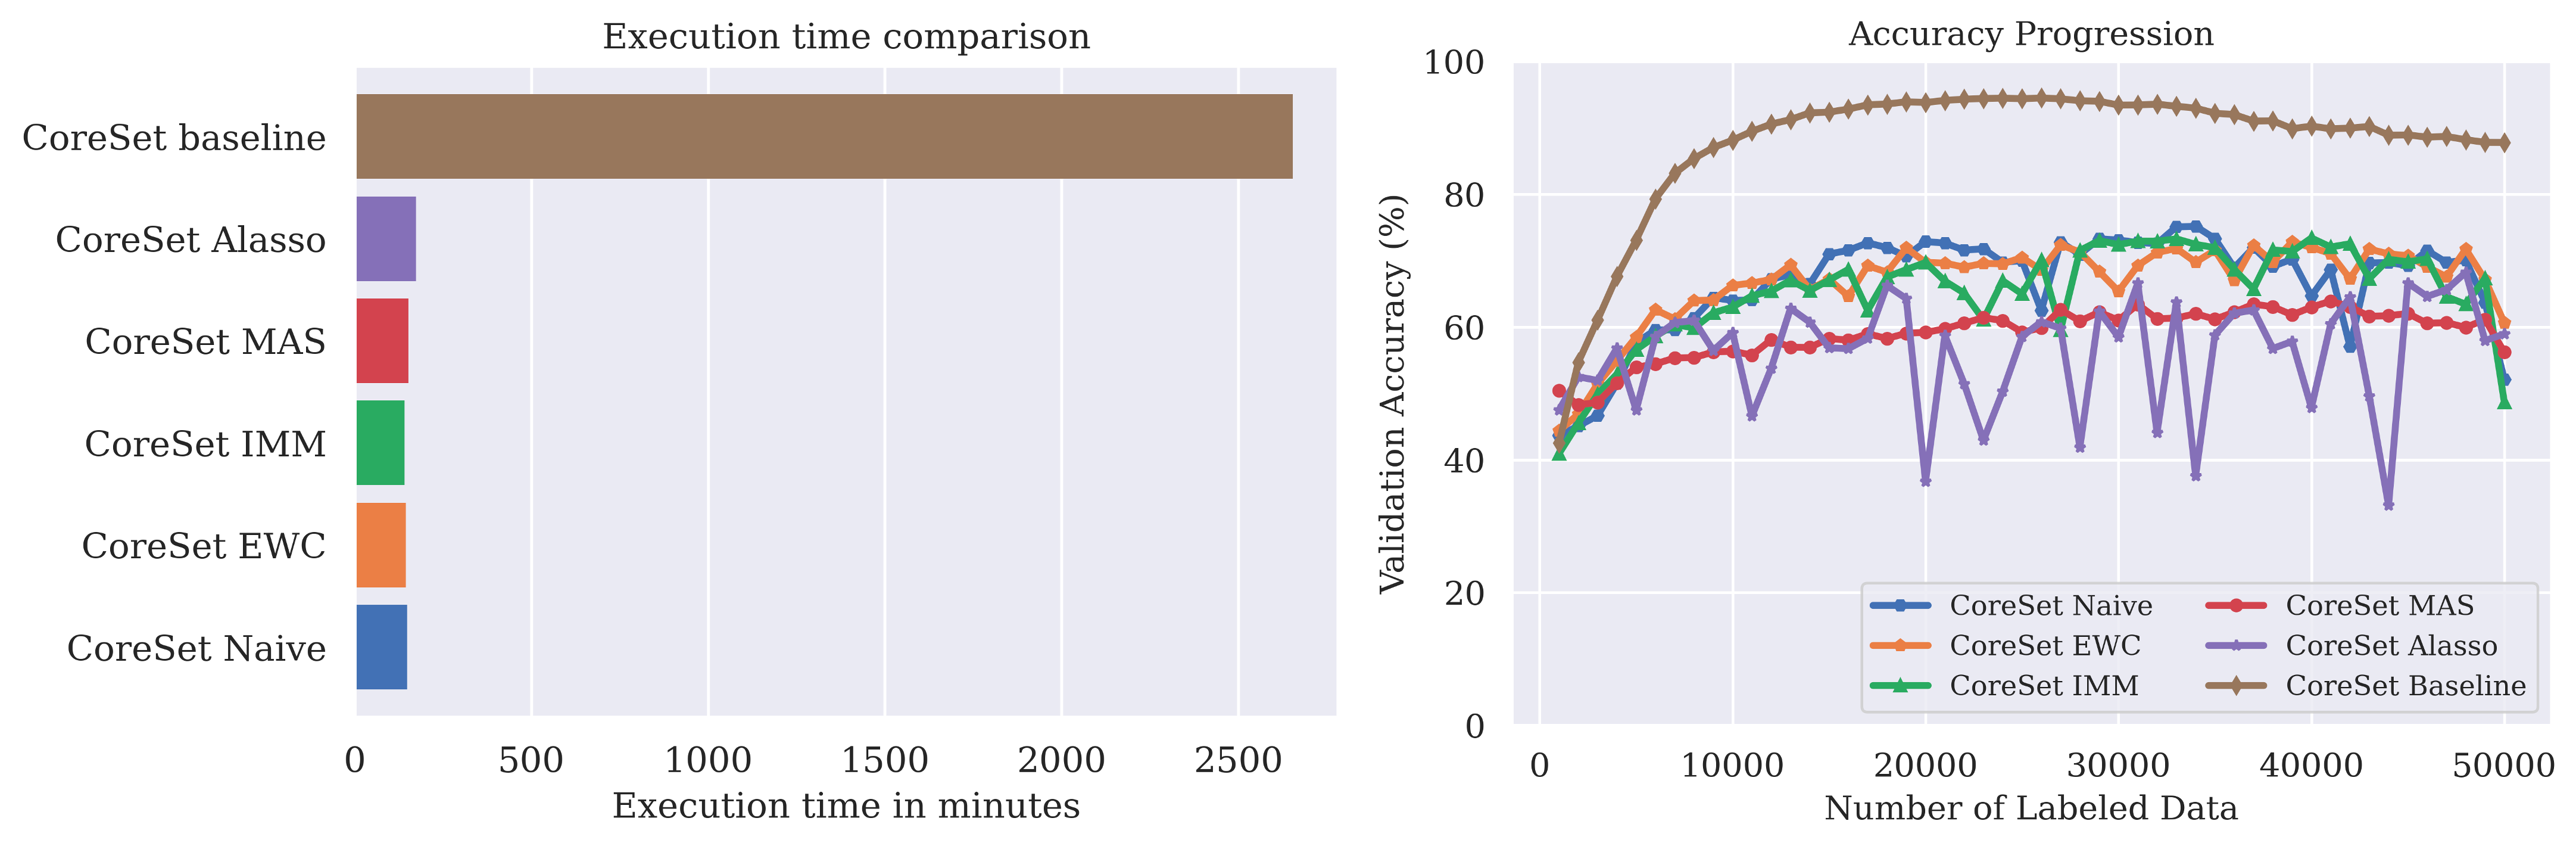
\includegraphics[width=\linewidth]{images/results_CAL/CoreSet_CAL_1000b.png}
    \caption[Continual Active Learning CoreSet 1000 batch size]{Comparison of execution time and validation accuracy of Continual Learning strategies used with the Active Learning strategy
     CoreSet. We use a batch size of 1000 for the experiments. }
    \label{fig:Evaluation:Results:CAL:CoreSet1000}
\end{figure}

% In terms of runtime, all
%     strategies are significantly faster than the classic Active Learning approach. However, there is a notable gap in validation accuracy between Active Learning and all Continual
%     Active Learning strategies. EWC performs best for the first 30000 samples but falls behind in the end. IMM performs closer to Naive with an increasing amount of samples. MAS and
%     Alasso perform significantly worse than the other strategies.
Badge: TO-DO when new plot is there

\begin{figure}[h]
    \centering
    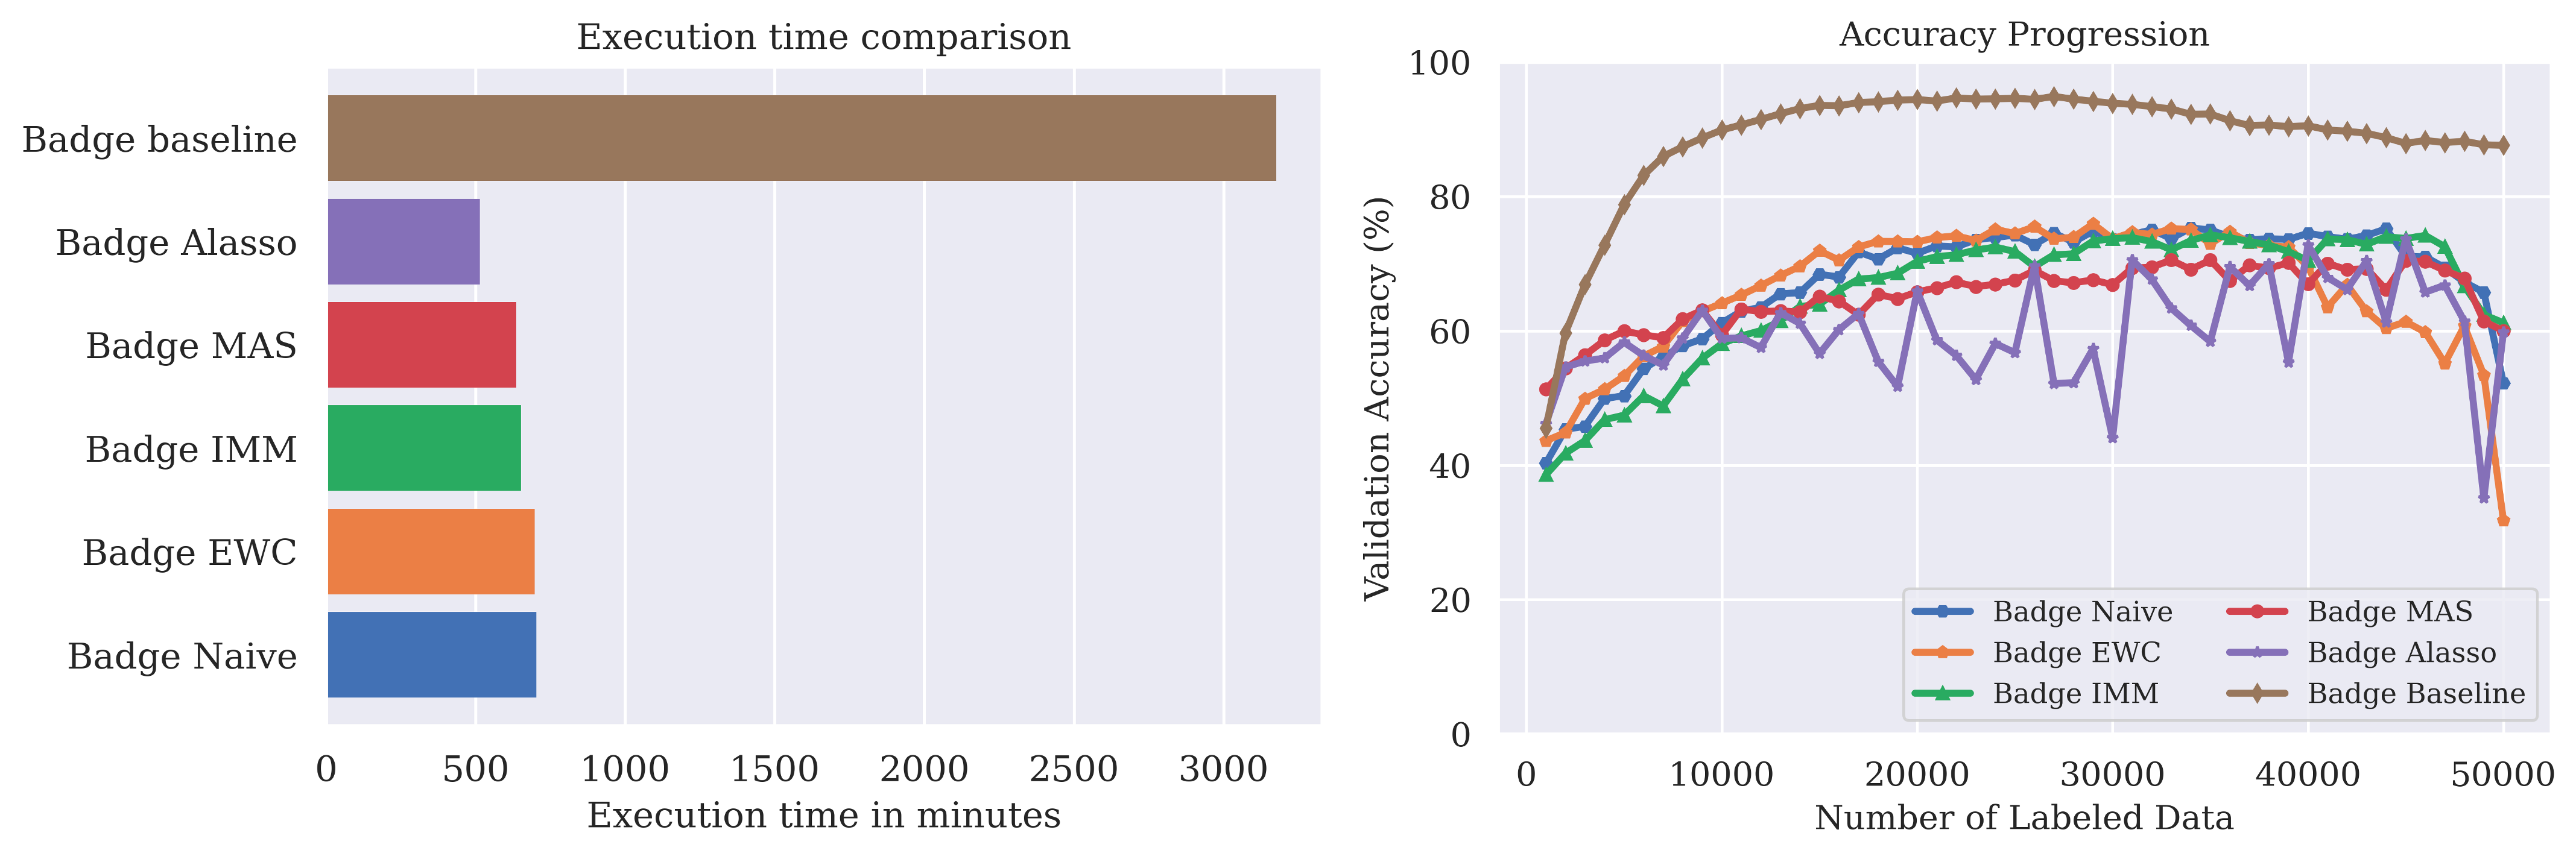
\includegraphics[width=\linewidth]{images/results_CAL/Badge_CAL_1000b.png}
    \caption[Continual Active Learning Badge 1000 batch size]{Comparison of execution time and validation accuracy of Continual Learning strategies used with the Active Learning strategy
    Badge. We use a batch size of 1000 for the experiments. }
    \label{fig:Evaluation:Results:CAL:Badge1000}
\end{figure}

After running the experiment with Badge, CoreSet, LC, BALD and Random, we perform the same experiment with Random but increase the batch size from 1000 to 2000. We present the results in
Figure \ref{fig:Evaluation:Results:CAL:Random2000}.The execution time remains significantly lower for all Continual Learning strategies compared to the baseline, however, the gap has decreased. 
Alasso is the slowest Continual Learning Strategy, being about 8 times as fast as the baseline. MAS, IMM, EWC and Naive have similar execution times, being about 10 times as fast as the baseline. 
The gap in validation accuracy between the baseline and the Continual Learning strategies is still significant, however, it has decreased compared the experiment with a batch size of 1000.
EWC outperforms all Continual Learning strategies, including Naive, although the gap between the two is marginal. Alasso, IMM and MAS perform show similar overall performance although the course
of their validation accuracy curves differ greatly. IMM starts worst and ends best. MAS shows similar performance to Alasso but is outperformed within the final 5000 samples. \par

\begin{figure}[h]
    \centering
    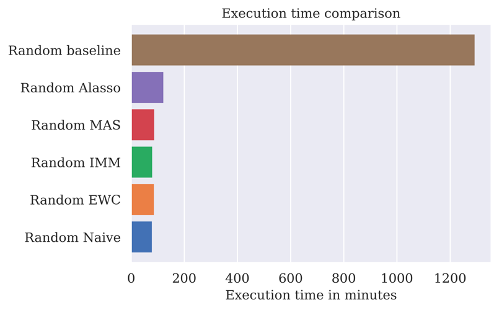
\includegraphics[width=\linewidth]{images/results_CAL/Random_CAL_2000b.png}
    \caption[Continual Active Learning Random 2000 batch size]{Comparison of execution time and validation accuracy of Continual Learning strategies used with the Active Learning strategy
    Random. We use a batch size of 2000 for the experiments.}
    \label{fig:Evaluation:Results:CAL:Random2000}
\end{figure}

Second, we run the experiment with batch size 2000 for the Active Learning strategy LC. Our results can be found in figure \ref{fig:Evaluation:Results:CAL:LC2000}. Like in the previous experiment,
the gap in execution time between the baseline and the Continual Learning strategies has shrunk compared to the experiment with a batch size of 1000. Again, Alasso is the slowest Continual Learning
strategy, being approximately 9 times as fast as the baseline. EWC is the second slowest strategy, being only marginally slower than MAS, IMM and Naive, who have a very similar execution time.
In terms of validation accuracy, there is still a significant gap between the baseline and the Continual Learning strategies. IMM, EWC and Naive perform similar for the first 35000 samples, outperforming
MAS and Alasso. In the final 15000 samples, all IMM, EWC and Naive experience a drop in validation accuracy, which is most significant for EWC. The accuracy of MAS increases modestly until the labeled
pool contains 40000 samples, before dropping of by about 10\%. The validation accuracy curve of Alasso is again unstable, showing a slight downward trend over the course of the experiment. \par

\begin{figure}[h]
    \centering
    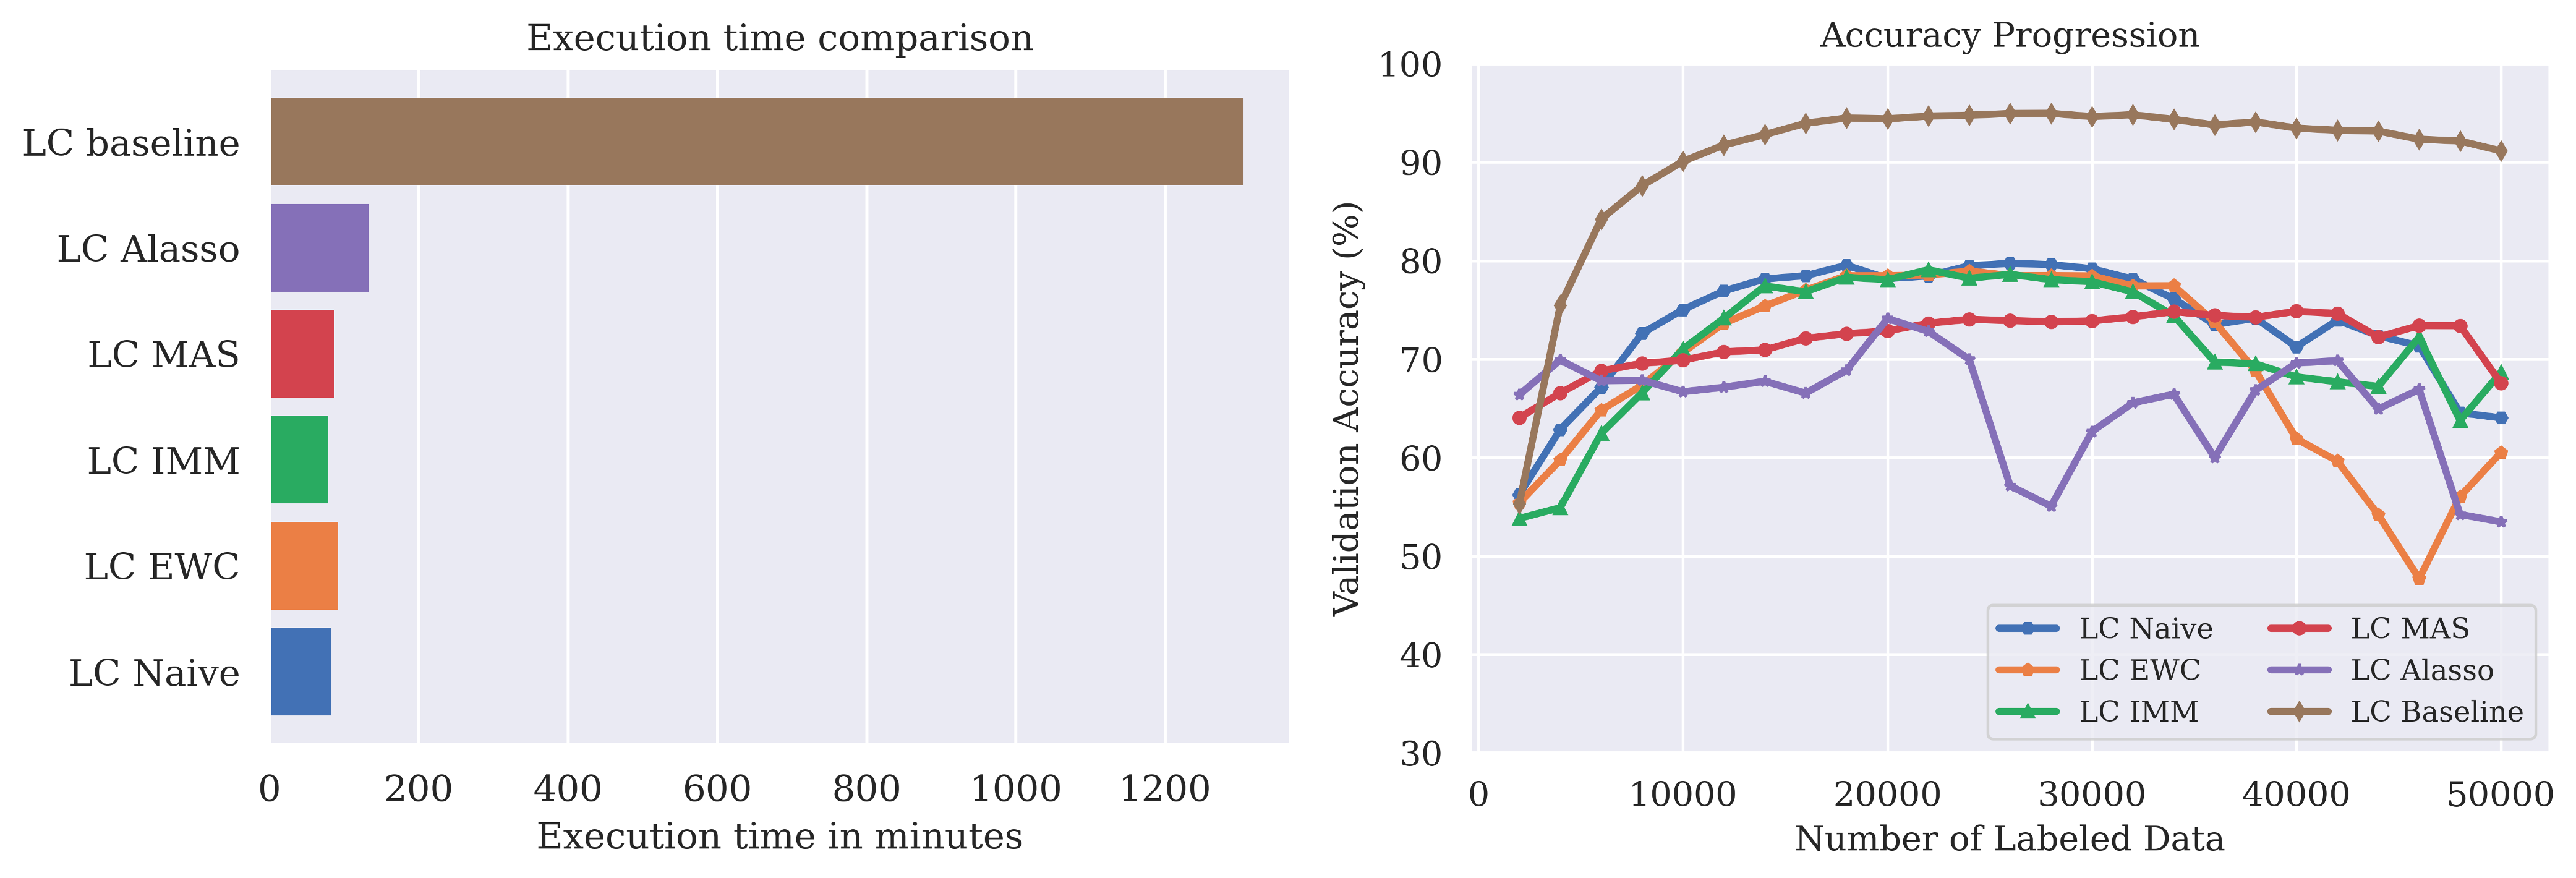
\includegraphics[width=\linewidth]{images/results_CAL/LC_CAL_2000b.png}
    \caption[Continual Active Learning LC 2000 batch size]{Comparison of execution time and validation accuracy of Continual Learning strategies used with the Active Learning strategy
    LC. We use a batch size of 2000 for the experiments.}
    \label{fig:Evaluation:Results:CAL:LC2000}
\end{figure}

We follow up with the experiment using the Active Learning strategy BALD, all other parameters being equal. The results can be found in figure \ref{fig:Evaluation:Results:CAL:BALD2000}. The gap in
execution time between the baseline and the Continual Learning strategies has declined compared to the experiment with BALD and batch size 1000. Naive and IMM are the fastest Continual Learning strategies,
closely followed EWC and MAS. Alasso follows last, but is still about 10 times as fast as the baseline. The validation accuracy curves of most Continual Learning strategies are similar, with Alasso falling 
out of line. EWC, IMM and Naive perform similar across the whole experiment with MAS starting off better but falling behind after approximately 15000 samples. Alasso performs on par with the remaining strategies
at first, but suffers from a heavy decrease in validation accuracy at around 15000 samples. All Continual Learning strategies leave a large gap to the baseline in terms of validation accuracy. \par

\begin{figure}[h]
    \centering
    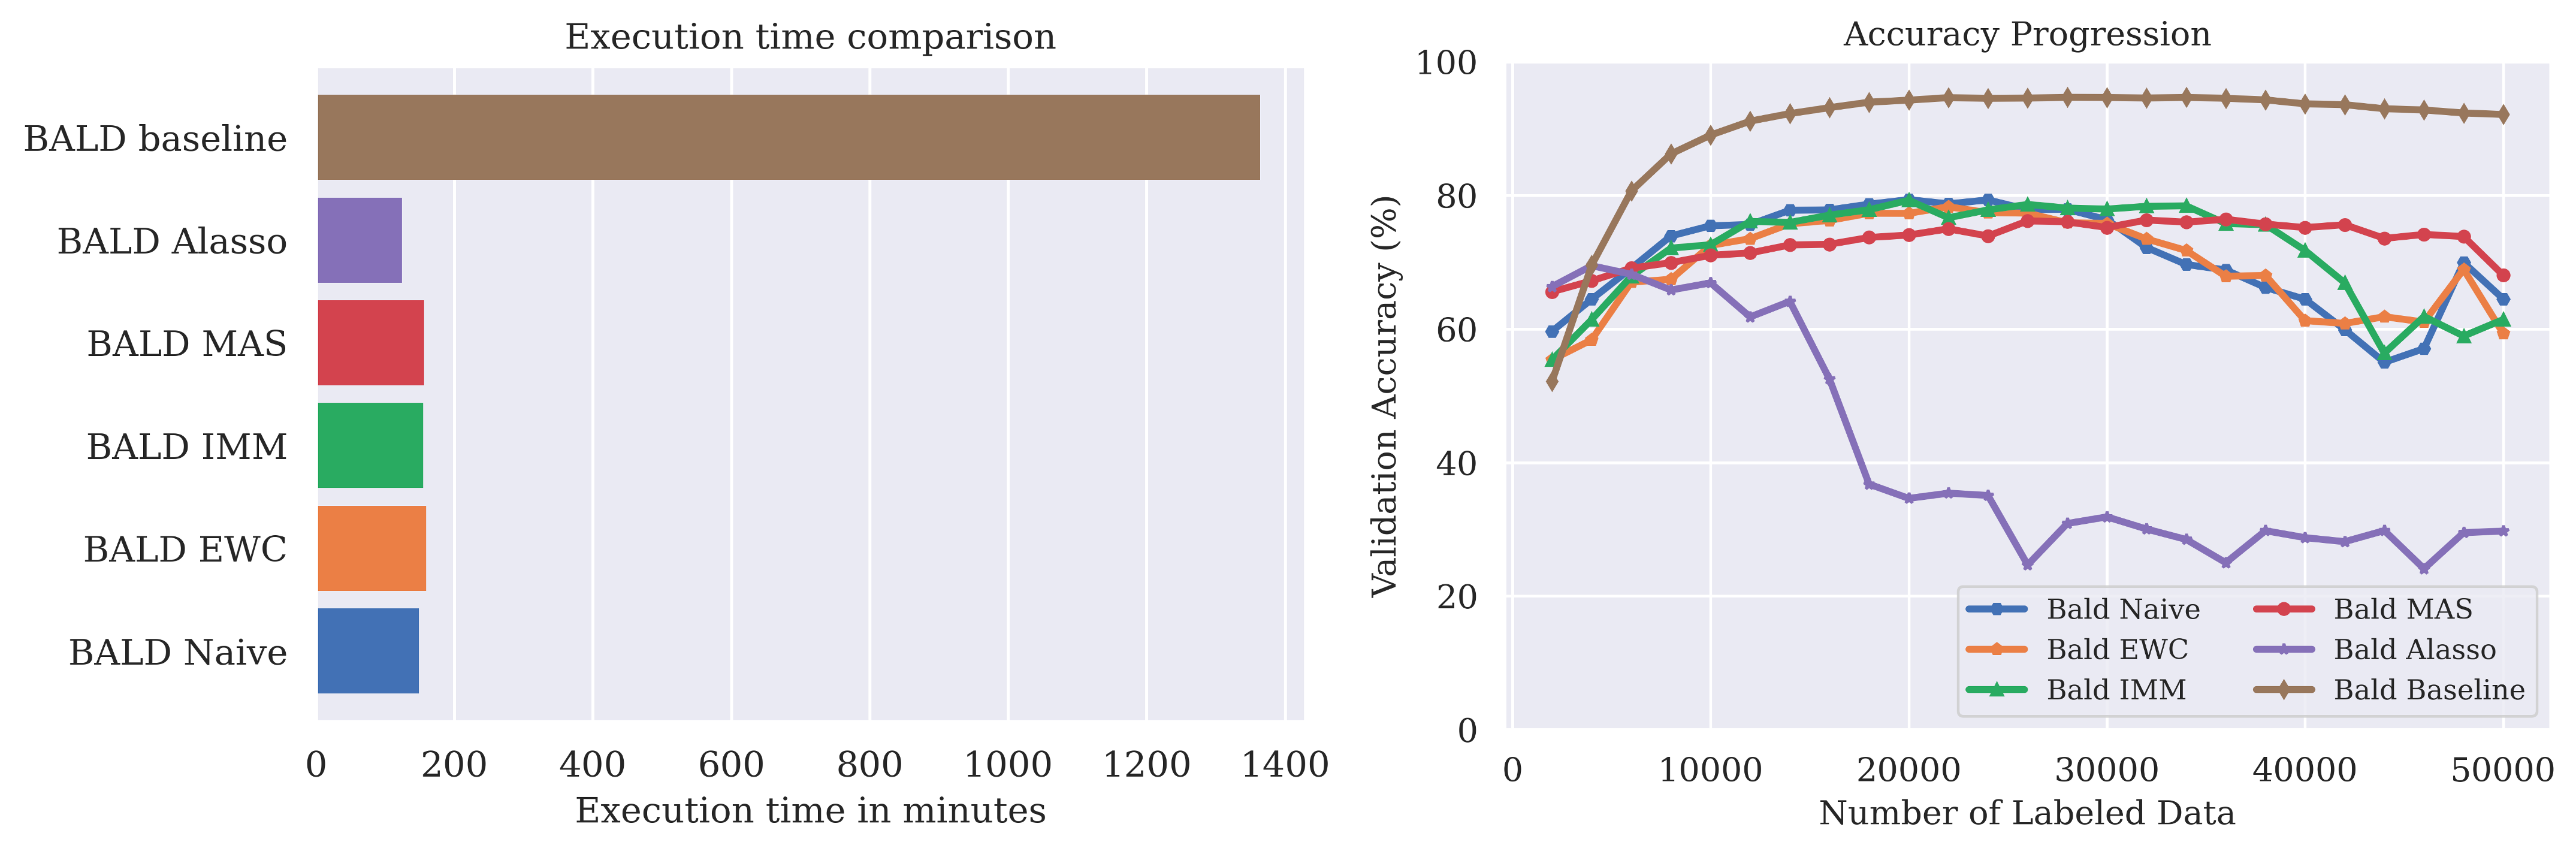
\includegraphics[width=\linewidth]{images/results_CAL/Bald_CAL_2000b.png}
    \caption[Continual Active Learning BALD 2000 batch size]{Comparison of execution time and validation accuracy of Continual Learning strategies used with the Active Learning strategy
    BALD. We use a batch size of 2000 for the experiments.}
    \label{fig:Evaluation:Results:CAL:BALD2000}
\end{figure}

%TODO
Next, we run the experiment with CoreSet and a batch size of 2000. We present our results in figure \ref{fig:Evaluation:Results:CAL:CoreSet2000}. The gap in execution time between the baseline and the
Continual Learning strategies has again decreased. IMM is the fastest Continual Learning strategy, closely followed by EWC. EWC is followed by Naive and MAS, who have similar execution times. Alasso is
the slowest approach, albeit being about 6.5 times as fast as the baseline. Regarding validation accuracy, all Continual Learning strategies are significantly outperformed by the baseline. Naive performs best
in the first half of the experiment, followed by EWC, IMM and MAS. At around 25000 samples, the validation accuracy of IMM, EWC and Naive suddenly becomes erratic, followed by a moderate increase in validation
accuracy and a drop in the final 10000 samples. MAS performs consistent but worse than IMM, EWC and Naive, experiencing a moderate drop in validation accuracy in the final 10000 samples. Alasso performs worst,
with its validation accuracy decreasing over the course of the experiment. \par

\begin{figure}[h]
    \centering
    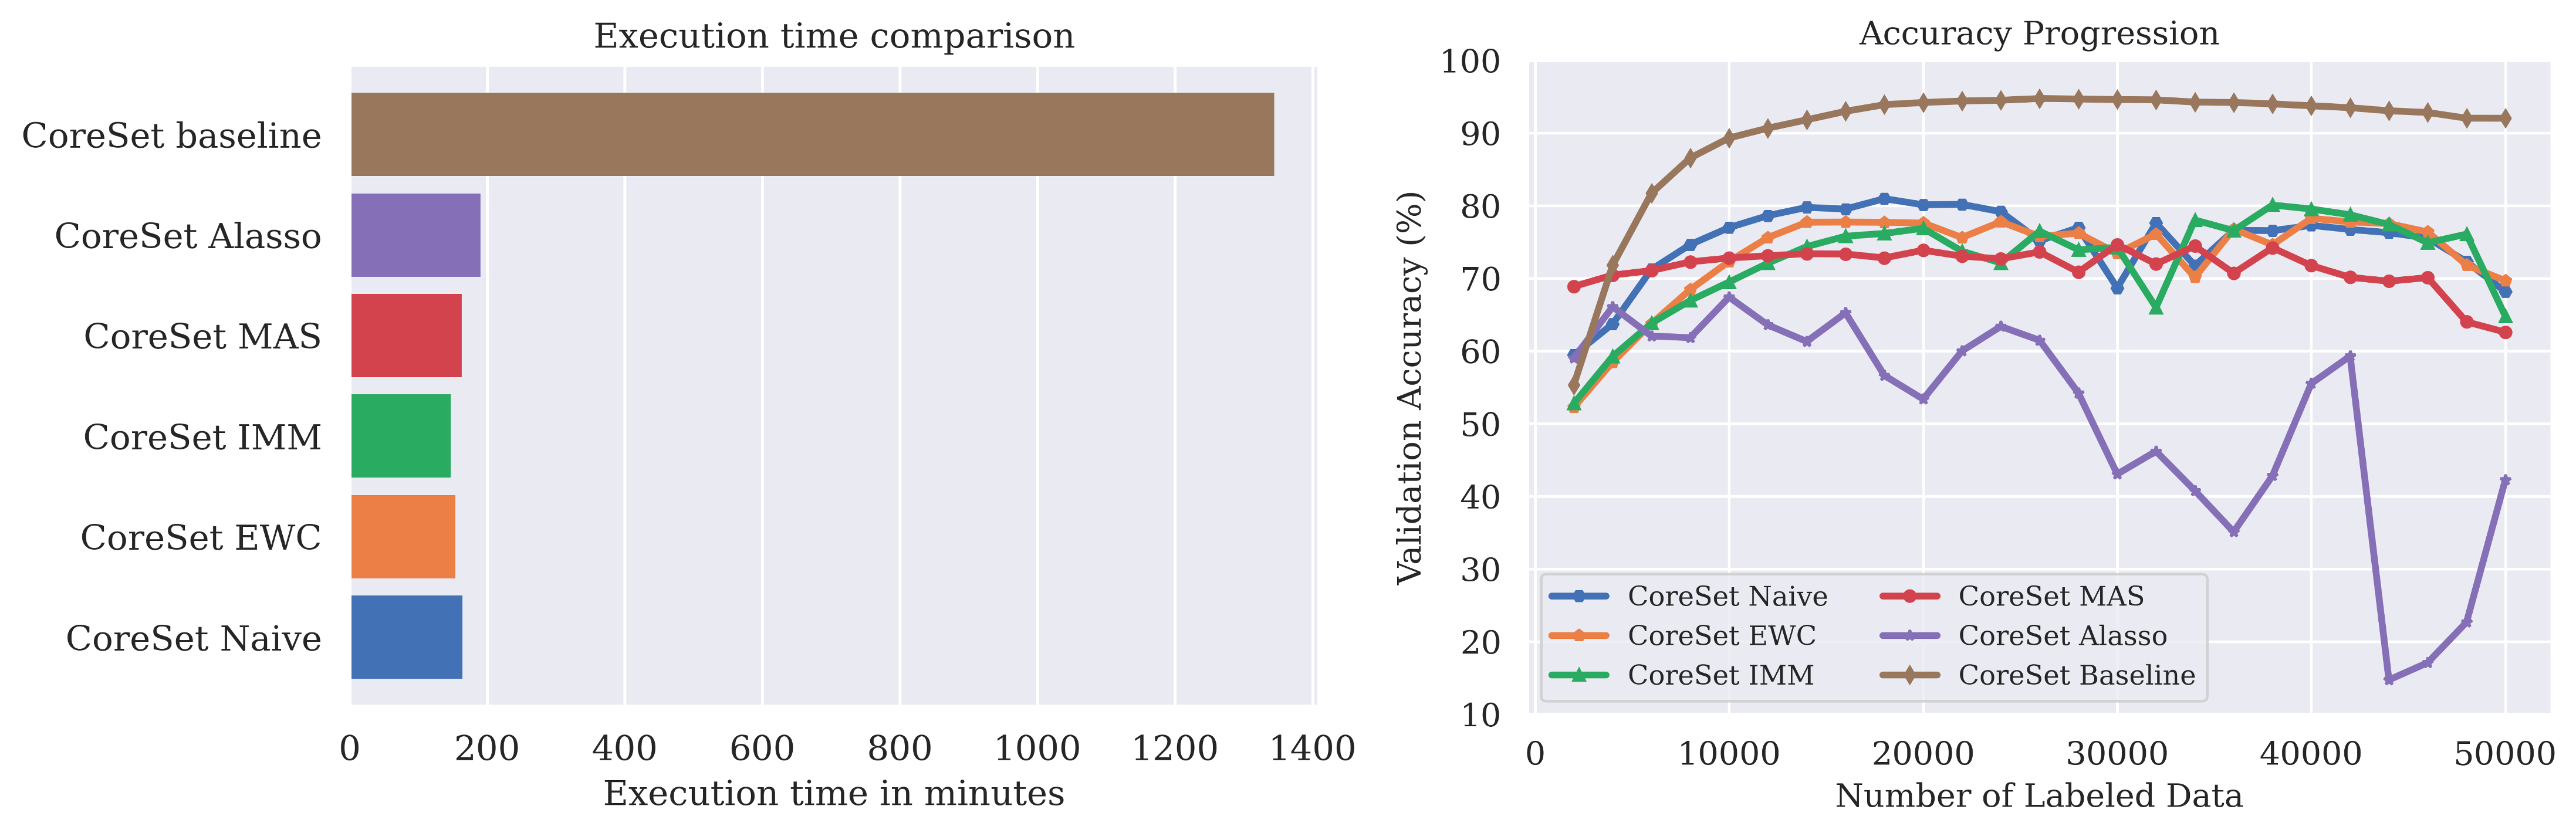
\includegraphics[width=\linewidth]{images/results_CAL/CoreSet_CAL_2000b.png}
    \caption[Continual Active Learning CoreSet 2000 batch size]{Comparison of execution time and validation accuracy of Continual Learning strategies used with the Active Learning strategy
    CoreSet. We use a batch size of 2000 for the experiments.}
    \label{fig:Evaluation:Results:CAL:CoreSet2000}
\end{figure}

%TODO
In terms of runtime, all
    strategies are 2.5-3 times faster than the classic Active Learning approach. However, there is a notable gap in validation accuracy between Active Learning and all Continual
    Active Learning strategies. The performance of IMM and EWC is similar to the Naive approach. MAS performs slightly worse than the first three, but 
    worse than the first three strategies but better than Alasso. The validation accuracy of Alasso becomes worse over time and is significantly worse than the other strategies.

\begin{figure}[h]
    \centering
    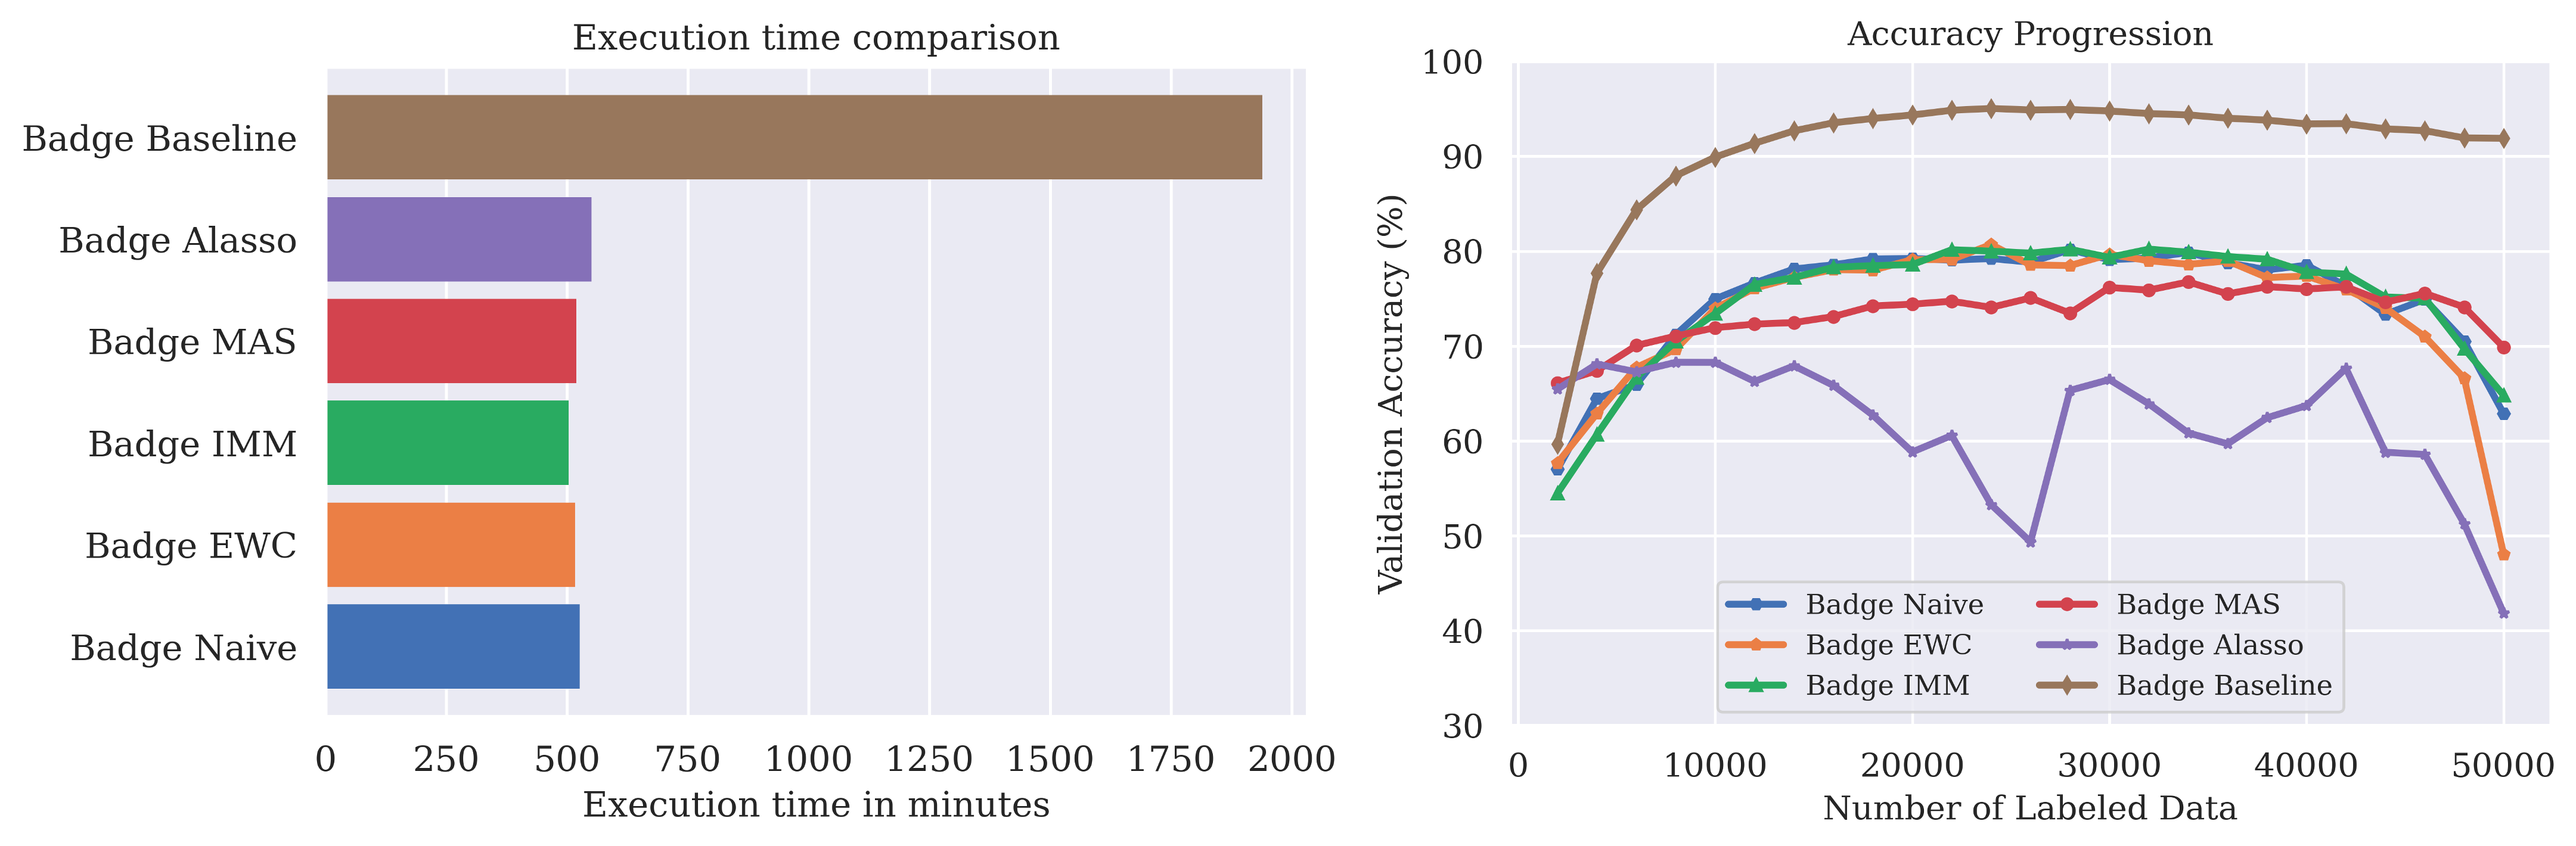
\includegraphics[width=\linewidth]{images/results_CAL/Badge_CAL_2000b.png}
    \caption[Continual Active Learning Badge 2000 batch size]{Comparison of execution time and validation accuracy of Continual Learning strategies used with the Active Learning strategy
    Badge. We use a batch size of 2000 for the experiments.}
    \label{fig:Evaluation:Results:CAL:Badge2000}
\end{figure}

Motivated by the increase in validation accuracy of the Continual Learning strategies with increasing batch size, we decide to re-run the experiments with a batch size of 4000. We start with the Active Learning
strategy Random. The results can be found in figure \ref{fig:Evaluation:Results:CAL:Random4000}. The gap in execution time between the baseline and the Continual Learning strategies has further decreased. IMM is
the fastest strategy, followed by MAS, EWC and Naive who perform on the same level in terms of execution time. Alasso is the slowest strategy, but is still about 6 times as fast as the baseline. There is still a
gap in validation accuracy between the baseline and the Continual Learning strategies, however it is smaller than in the experiment with batch size 2000. Overall, EWC and Naive perform best, followed by IMM and MAS.
Alasso starts of as the best strategy but suffers from a heavy decrease in validation accuracy, starting at around 8000 samples. \par

\begin{figure}[h]
    \centering
    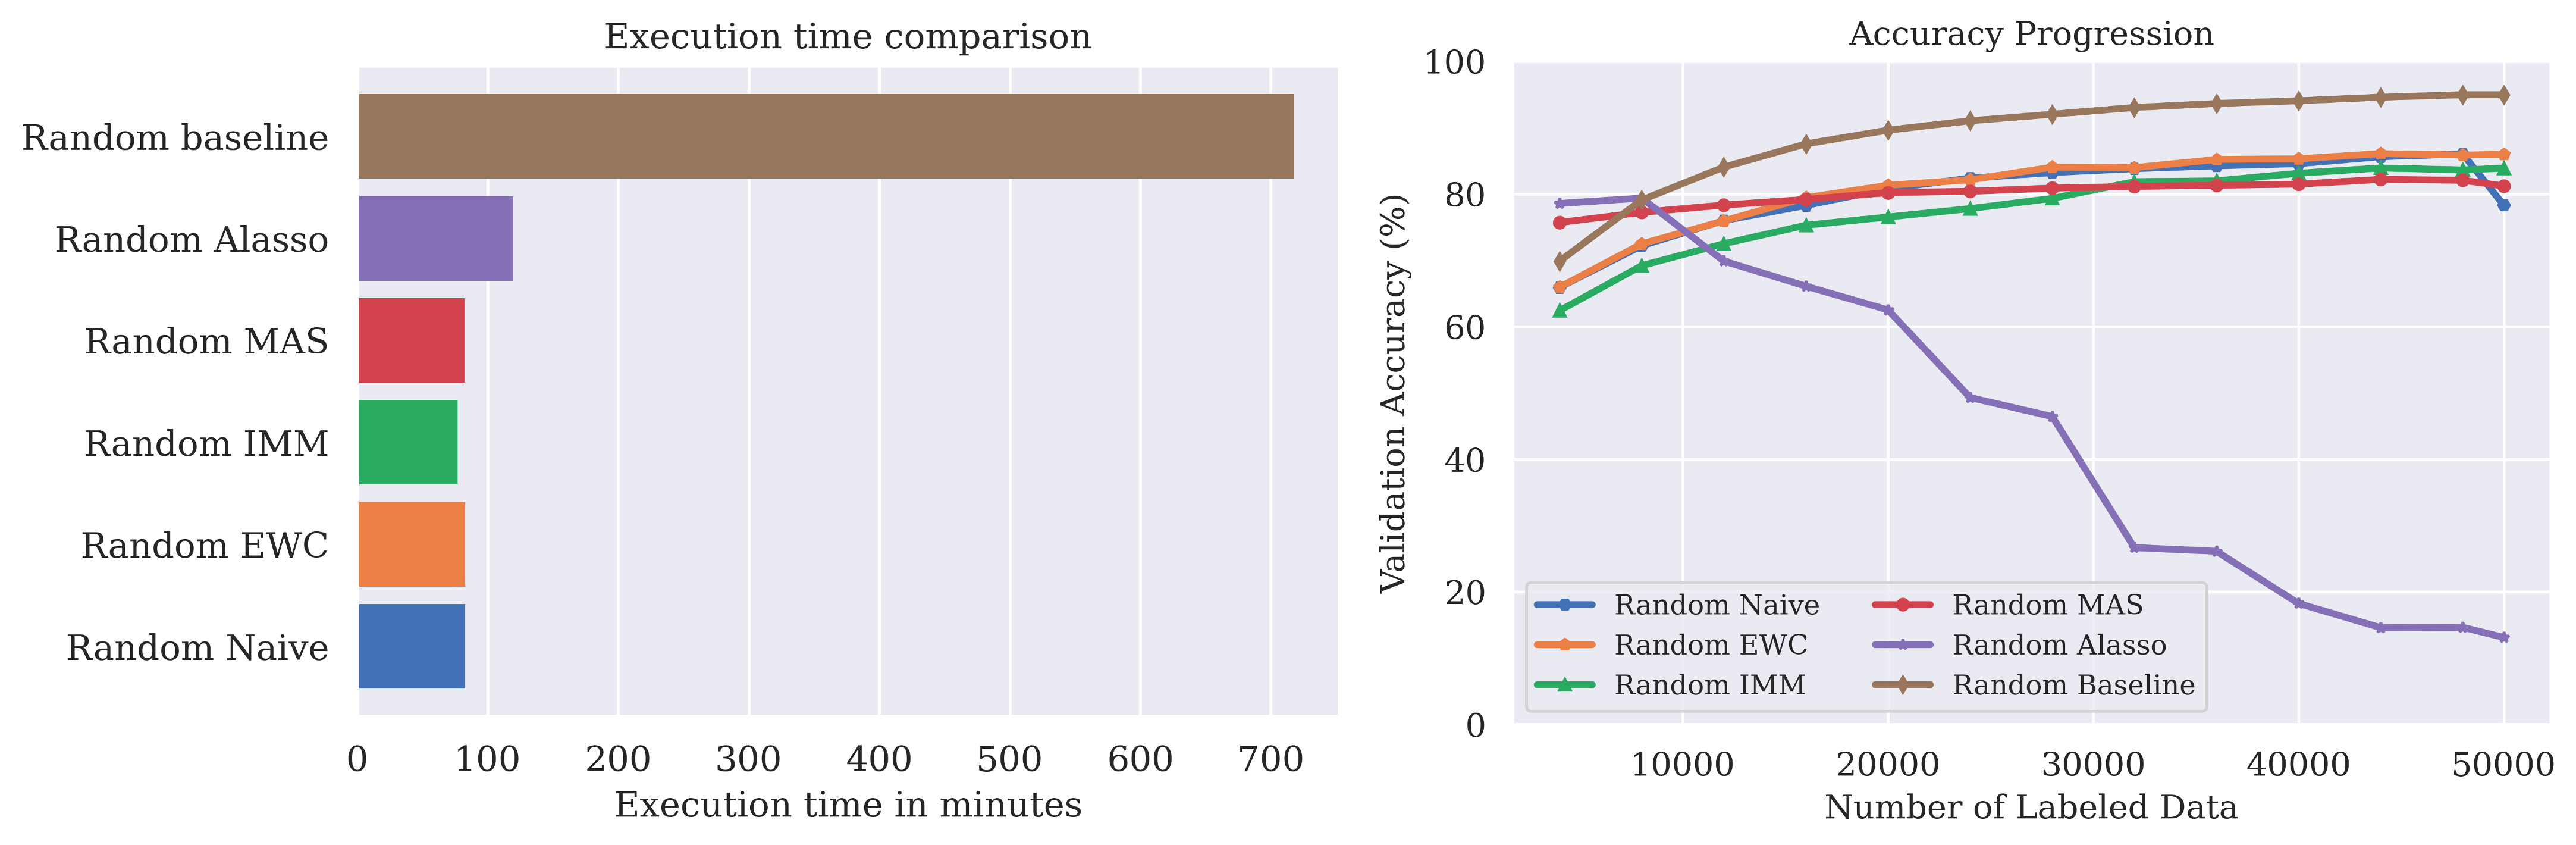
\includegraphics[width=\linewidth]{images/results_CAL/Random_CAL_4000b.png}
    \caption[Continual Active Learning Random 4000 batch size]{Comparison of execution time and validation accuracy of Continual Learning strategies used with the Active Learning strategy
    Random. We use a batch size of 4000 for the experiments}
    \label{fig:Evaluation:Results:CAL:Random4000}
\end{figure}

Next, we re-run the previous experiment with the Active Learning strategy LC, again using a batch size of 4000. We present the results of the experiment in Figure \ref{fig:Evaluation:Results:CAL:LC4000}. In terms of runtime,
the results are similar to the experiment with Random, with Alasso being the slowest Continual Learning strategy, followed by MAS, EWC, IMM and Naive. All Continual Learning strategies are significantly faster than the baseline,
with Alasso being about 6 times as fast and Naive about 10 times as fast. The gap in validation accuracy between the baseline and the Continual Learning strategies remains significant, although it has shrunk compared to the
experiment with 2000 batch size. IMM, EWC and Naive perform almost identically across the experiment with MAS following closely and outperforming the remaining strategies within the last 5000 samples. Alasso starts of on par
with the remaining strategies, but suffers from a heavy decrease in validation accuracy at around 8000 samples. \par

\begin{figure}[h]
    \centering
    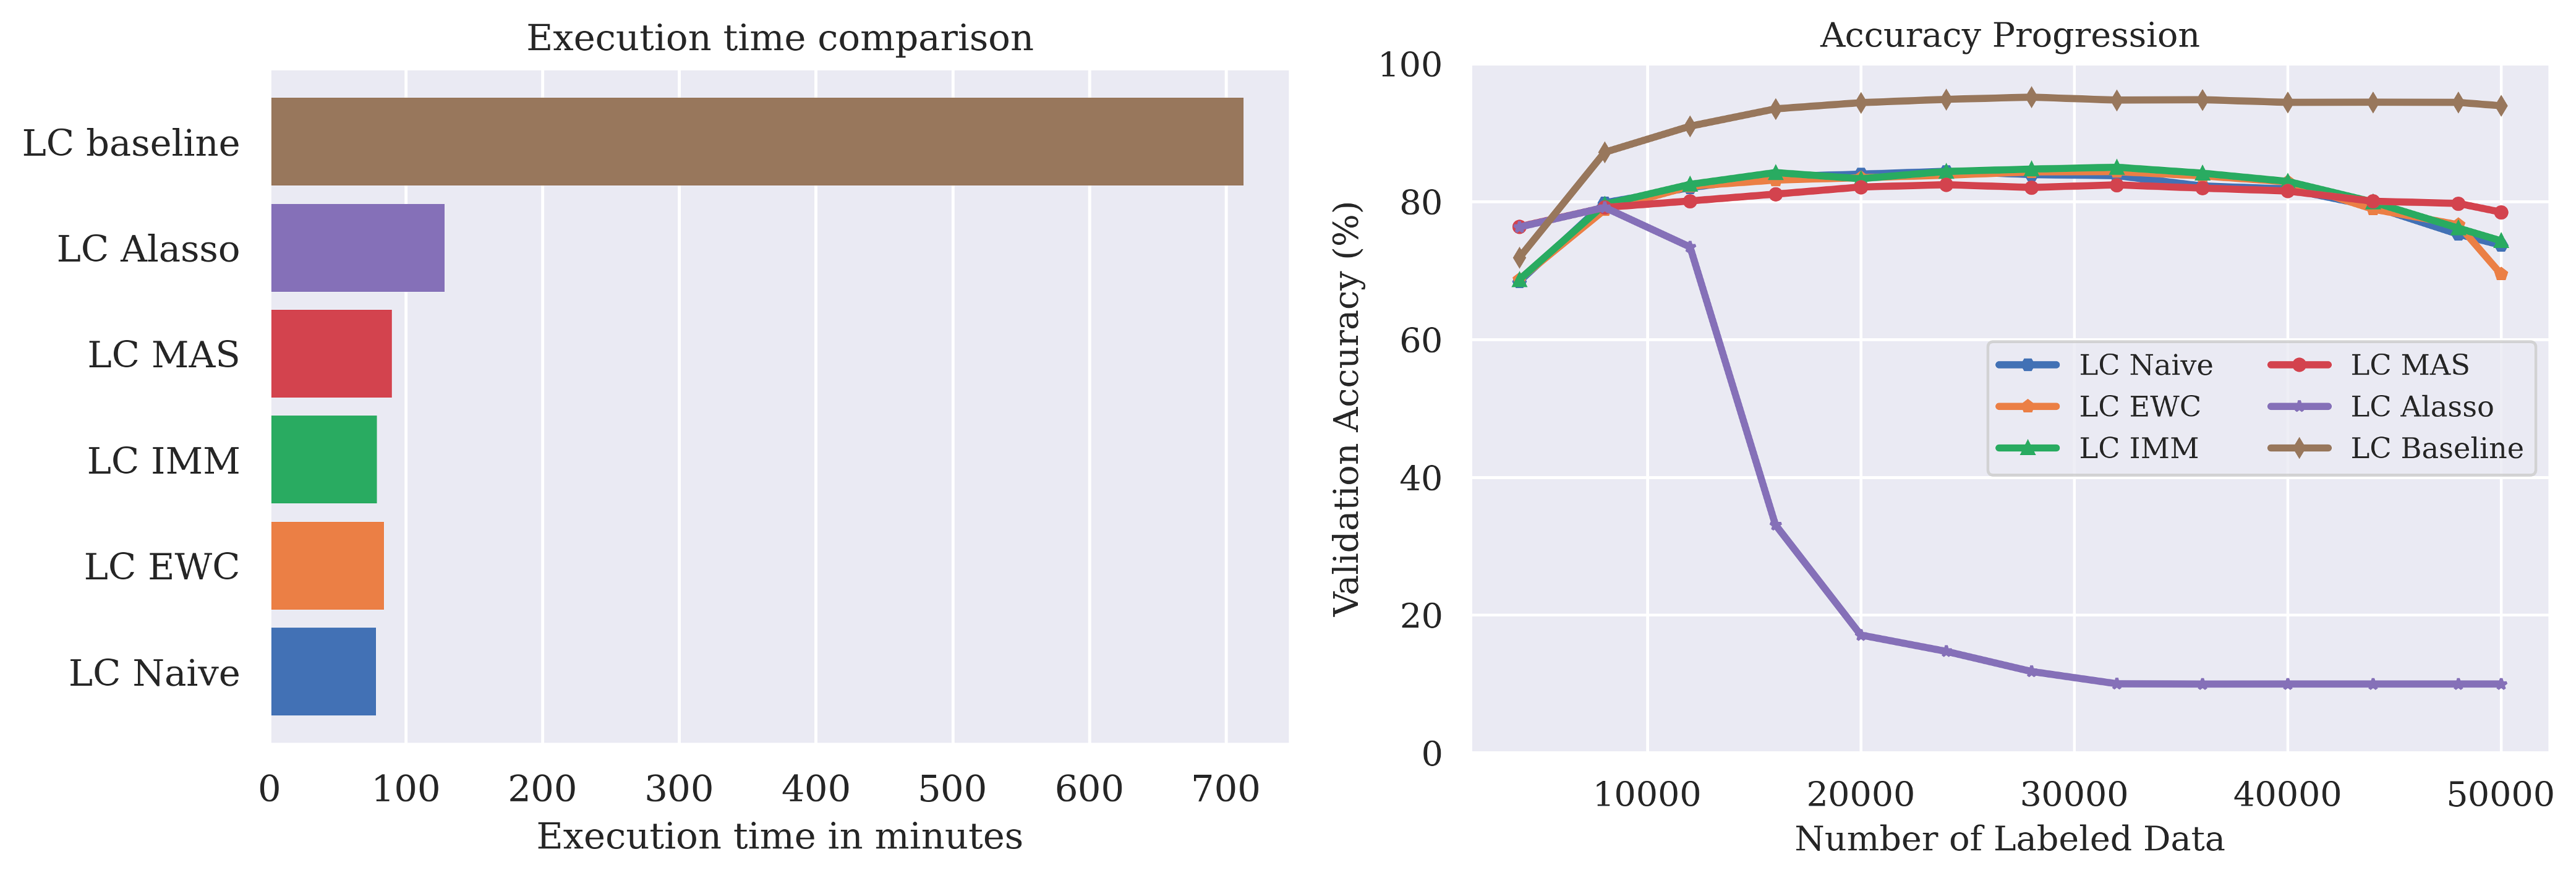
\includegraphics[width=\linewidth]{images/results_CAL/LC_CAL_4000b.png}
    \caption[Continual Active Learning LC 4000 batch size]{Comparison of execution time and validation accuracy of Continual Learning strategies used with the Active Learning strategy
    LC. We use a batch size of 4000 for the experiments. }
    \label{fig:Evaluation:Results:CAL:LC4000}
\end{figure}

The third experiment with a batch size of 4000 is run with the Active Learning strategy BALD. The results of the experiment can be found in figure \ref{fig:Evaluation:Results:CAL:BALD4000}. The ranking of execution time of the Continual
Learning strategies and the baseline is similar to the previous experiment with LC. In terms of accuracy, there remains a large gap between the baseline and all Continual Learning strategies. Naive, IMM and EWC perform similar, showing an
s-shaped validation accuracy curve. The performance of MAS follows a similar curve, however MAS performs better in the first half of the experiment, and worse in the second half compared to the three former strategies. Alasso starts off as
the best Continual Learning strategy, but its validation accuracy decreases steadily over the course of the experiment, until it suffers a huge drop in the final iteration. \par 

\begin{figure}[h]
    \centering
    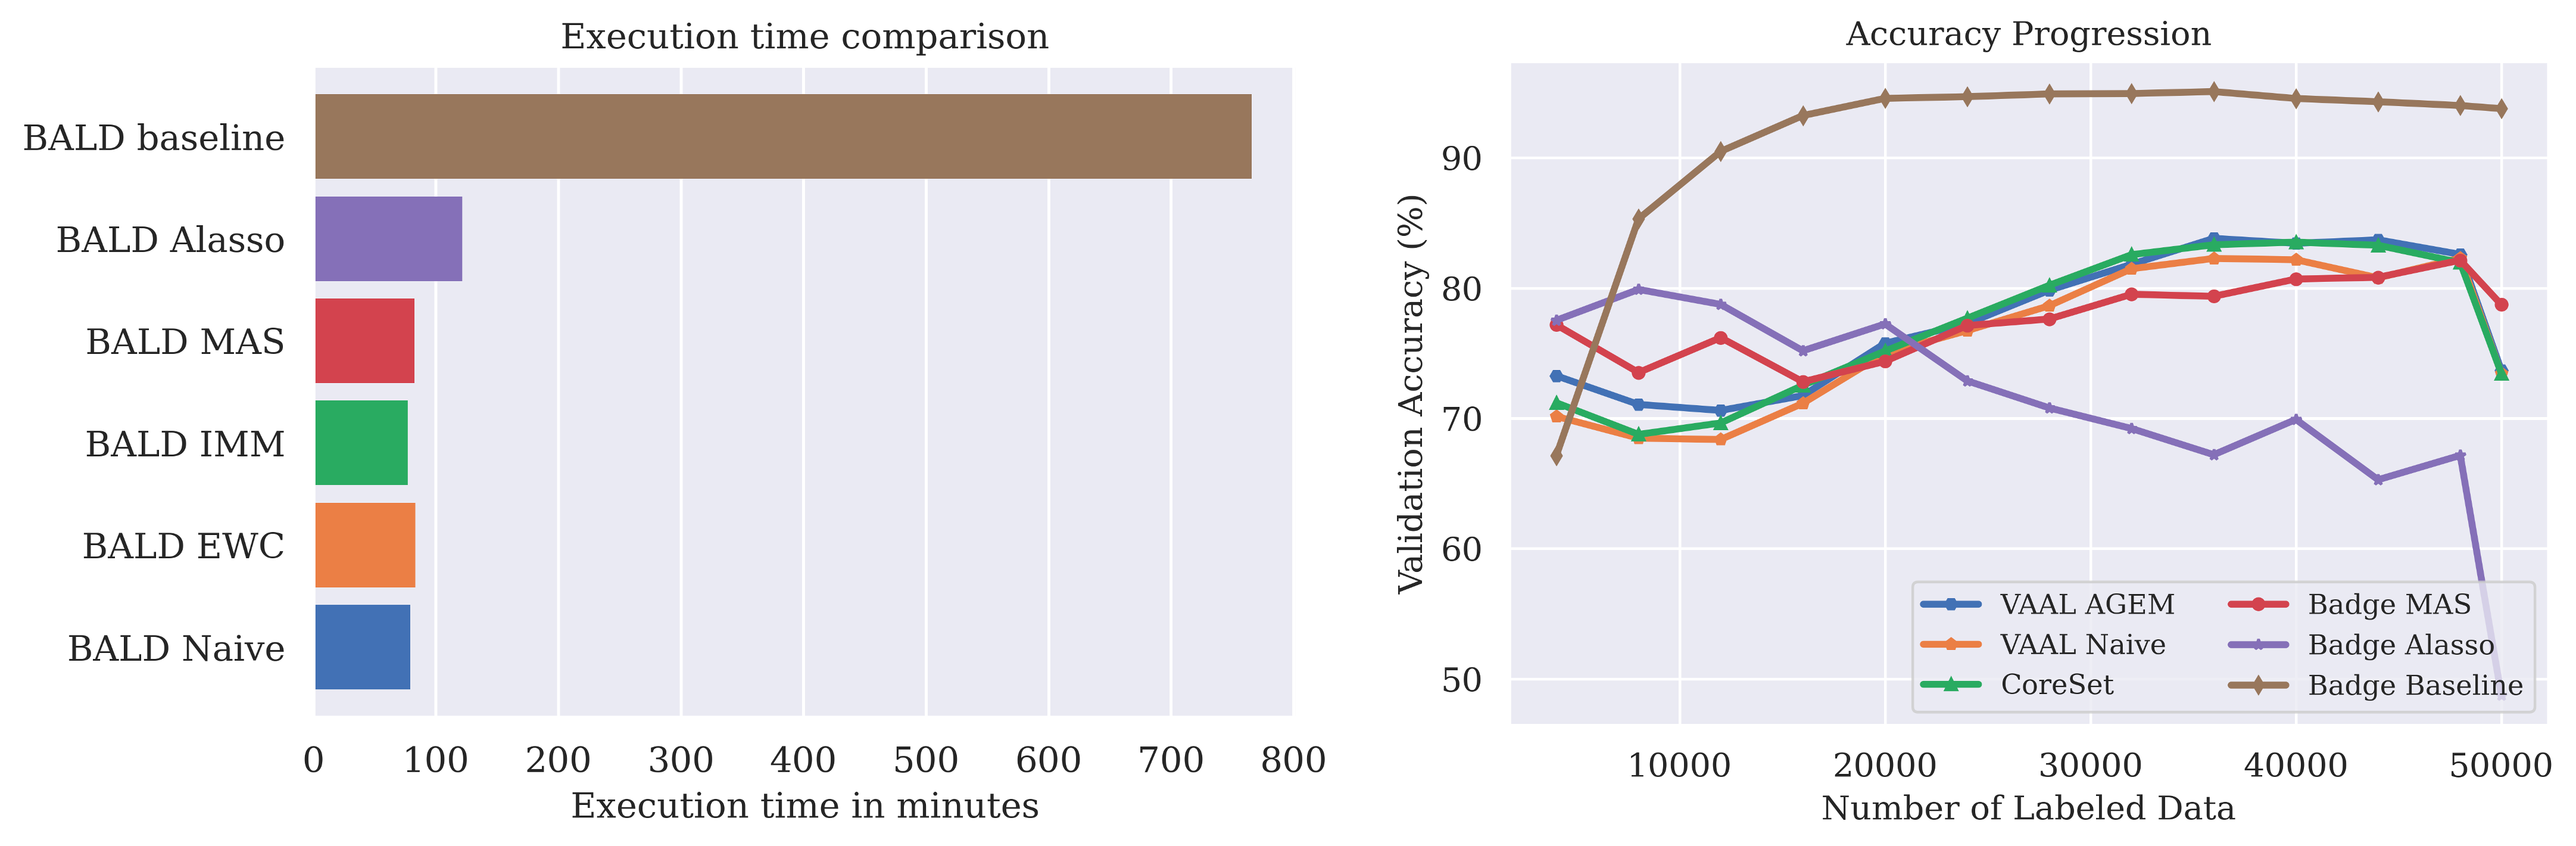
\includegraphics[width=\linewidth]{images/results_CAL/Bald_CAL_4000b.png}
    \caption[Continual Active Learning BALD 4000 batch size]{Comparison of execution time and validation accuracy of Continual Learning strategies used with the Active Learning strategy
    BALD. We use a batch size of 4000 for the experiments }
    \label{fig:Evaluation:Results:CAL:BALD4000}
\end{figure}

%TODO

We now run the experiment with the identical setup with the Active Learning strategy CoreSet. Our results are presented in figure \ref{fig:Evaluation:Results:CAL:CoreSet4000}. The gap in execution time between the baseline and the Continual Learning 
strategies has further decreased. IMM is the fastest Continual Learning strategy, being about 6 times as fast as the baseline. On the other hand, Alasso is the slowest Continual Learning strategy, boasting around one fourth of the execution time of the
baseline. Not only the gap in execution time has decreased compared to the experiment with batch size 2000, but also the gap in validation accuracy. Naive is the best performing strategy, lacking only 10 percentage points in validation accuracy to the
baseline during the first half of the experiment. IMM, EWC and MAS follow in that order, showing a similar validation accuracy curve as Naive. Alasso starts with a similar validation accuracy as the other Continual Learning strategies, but falls behind
after 8000 samples. \par


\begin{figure}[h]
    \centering
    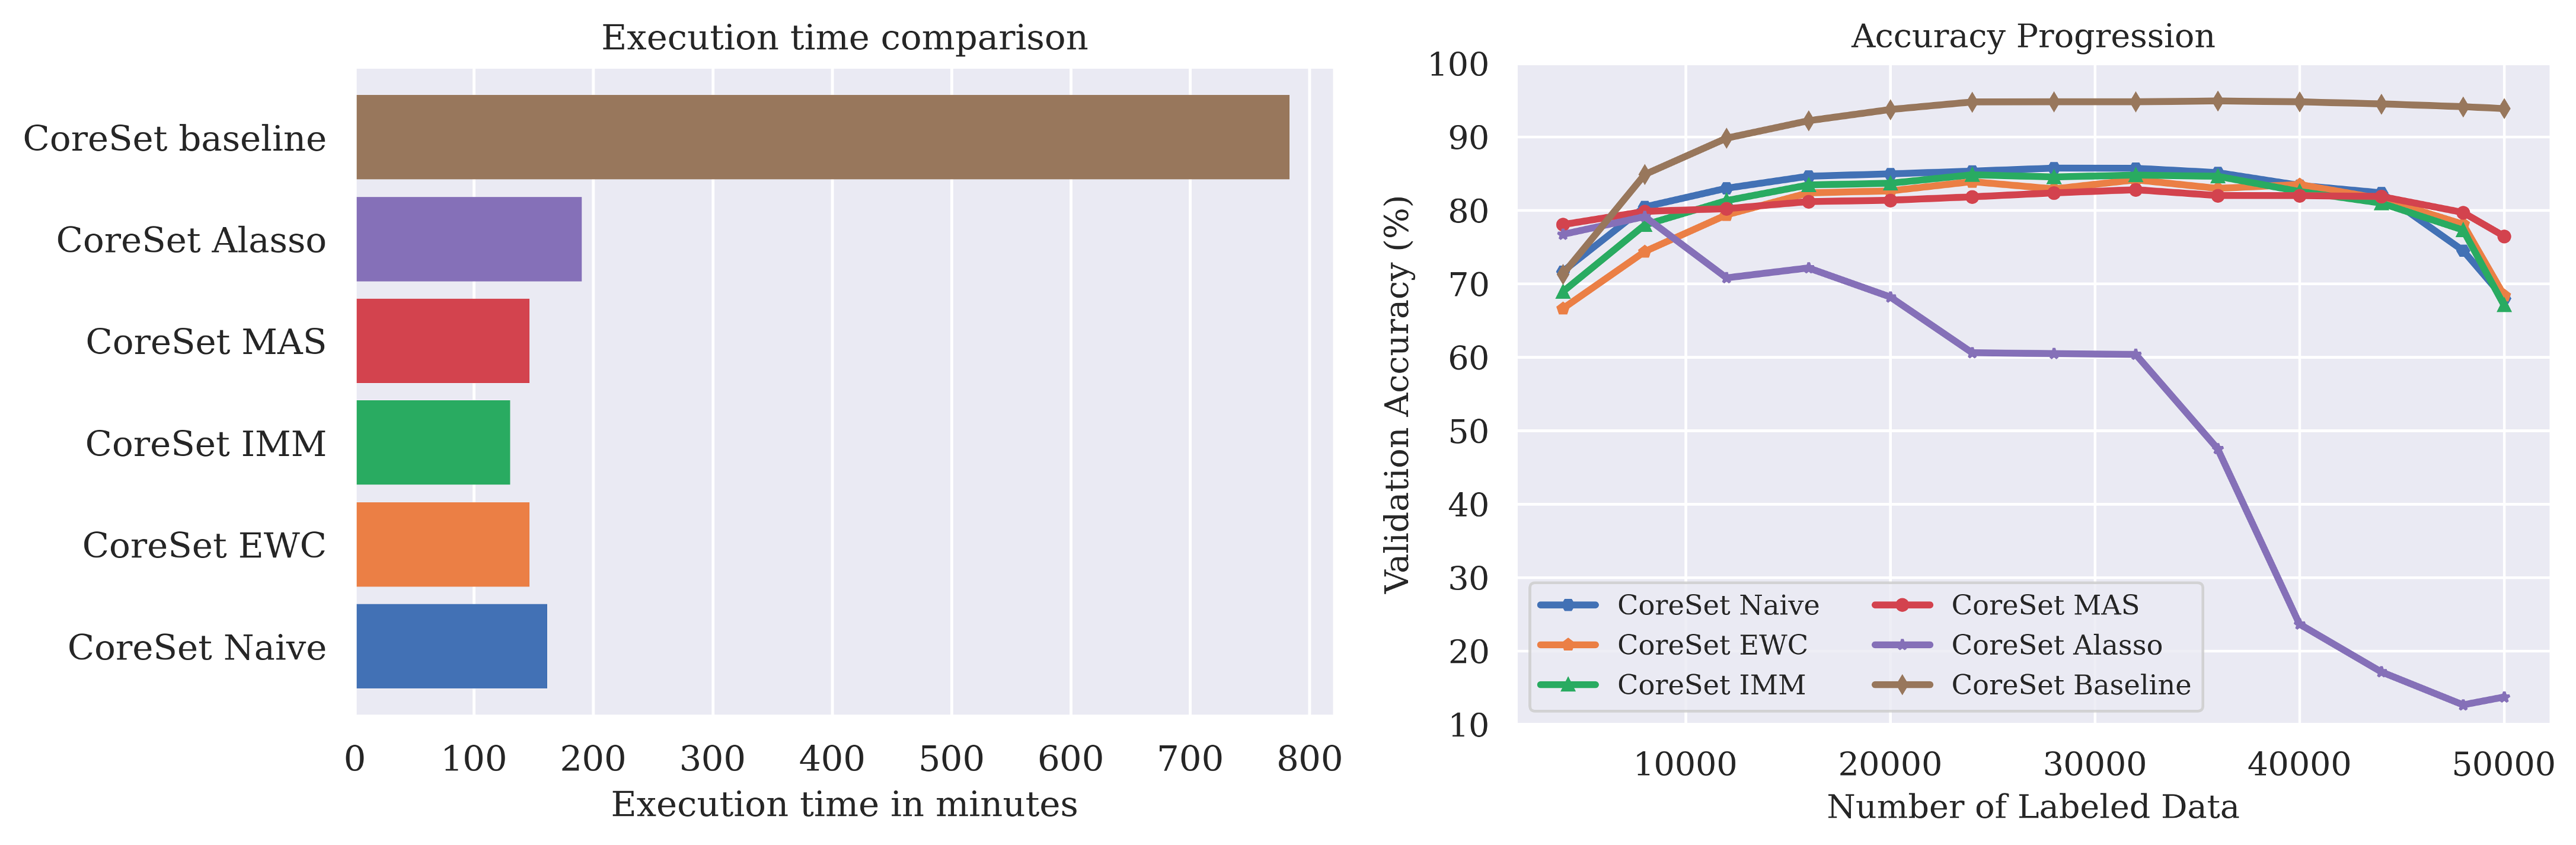
\includegraphics[width=\linewidth]{images/results_CAL/CoreSet_CAL_4000b.png}
    \caption[Continual Active Learning CoreSet 4000 batch size]{Comparison of execution time and validation accuracy of Continual Learning strategies used with the Active Learning strategy
    CoreSet. We use a batch size of 4000 for the experiments.}
    \label{fig:Evaluation:Results:CAL:CoreSet4000}
\end{figure}

%TODO
In terms of runtime, all
    strategies are approximately 2 times faster than the classic Active Learning approach. There is a gap in validation accuracy between Active Learning and all Continual
    Active Learning strategies, however this is lower than the gap for smaller batch sizes. The Naive approach performs best, closely followed by EWC. IMM comes third decreasing the
    performance gap to the third two approaches with increasing number of labeled data. MAS follows IMM and Alasso falls behind significantly.

\begin{figure}[h]
    \centering
    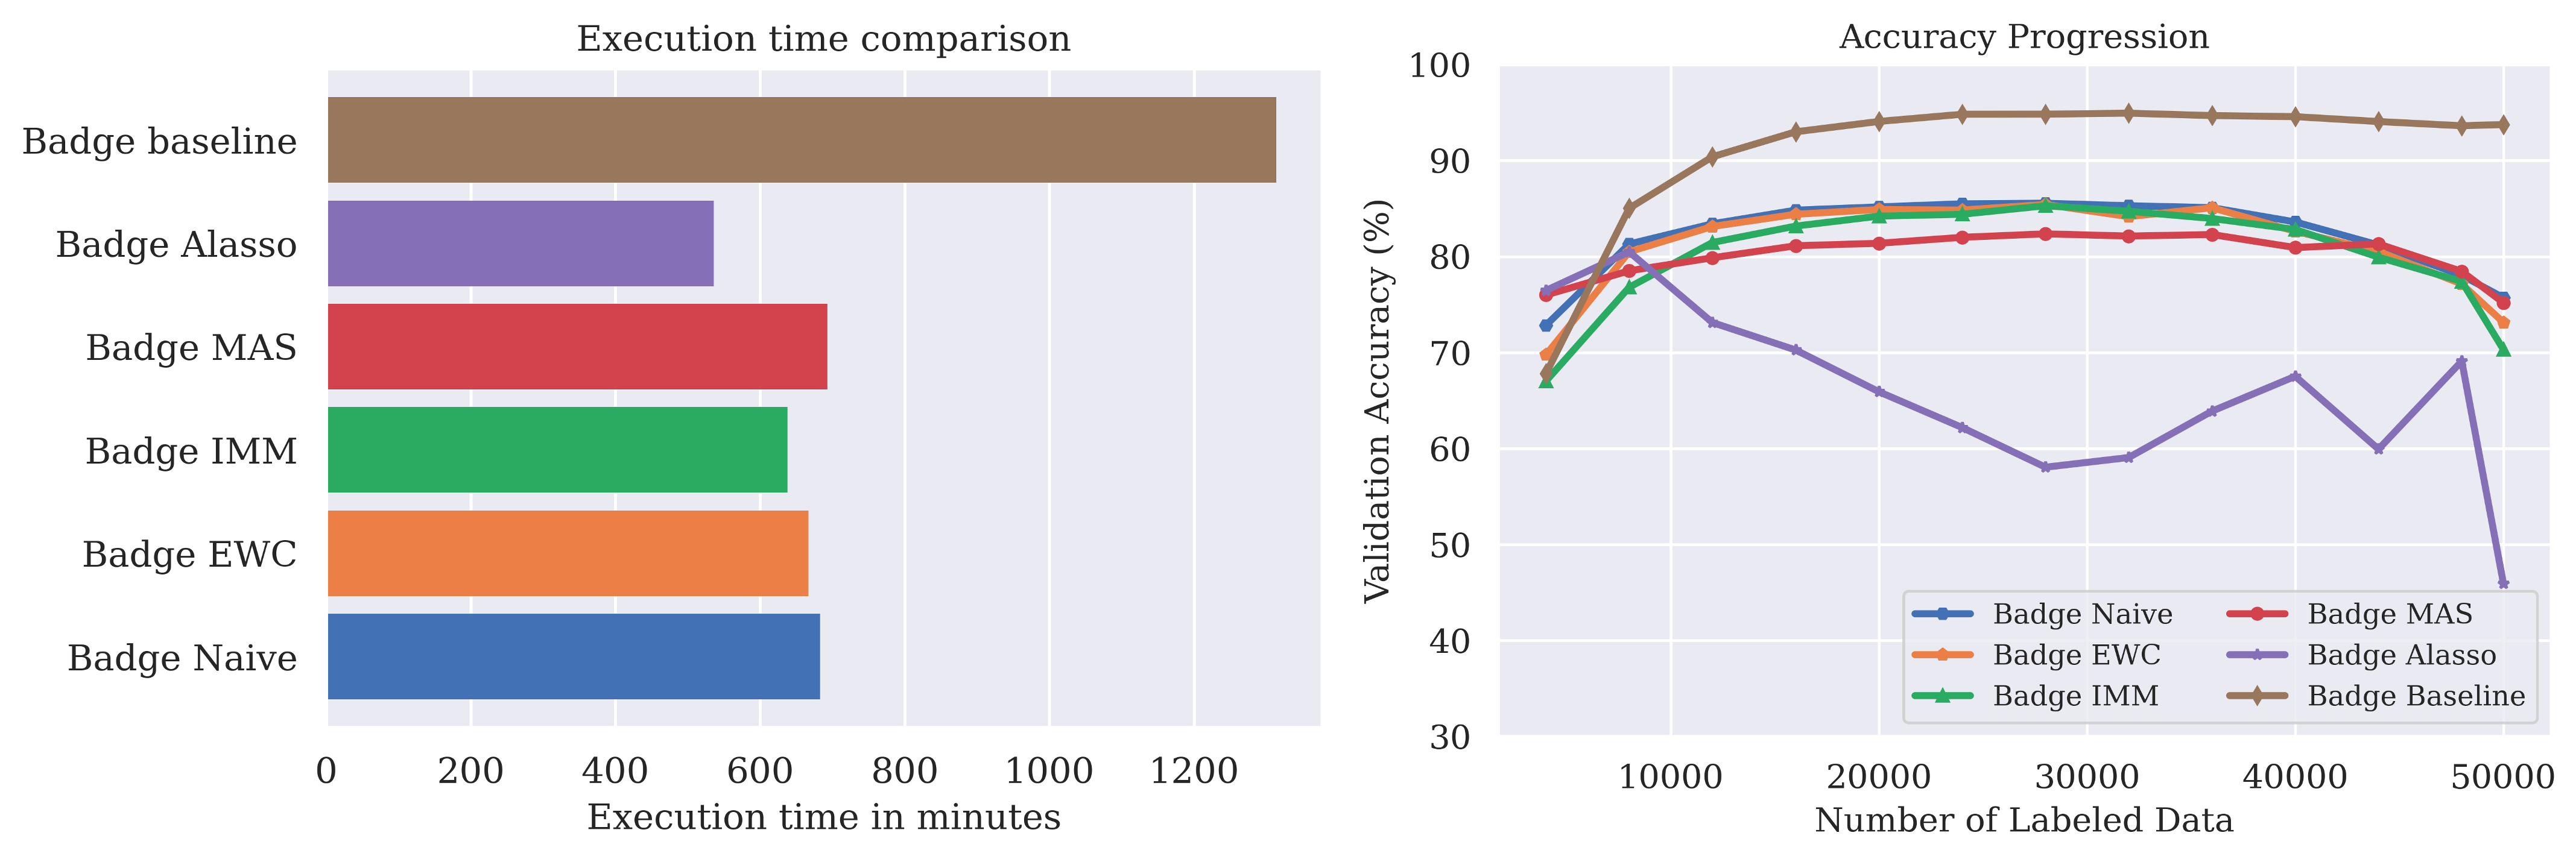
\includegraphics[width=\linewidth]{images/results_CAL/Badge_CAL_4000b.png}
    \caption[Continual Active Learning Badge 4000 batch size]{Comparison of execution time and validation accuracy of Continual Learning strategies used with the Active Learning strategy
    Badge. We use a batch size of 4000 for the experiments.}
    \label{fig:Evaluation:Results:CAL:Badge4000}
\end{figure}

\subsubsection{A hybrid approach to Continual Learning}
\label{sec:Evaluation:Results:CAL:Hybrid}
After running the experiments in section \ref{sec:Evaluation:Results:CAL:ALCL}, we notice that all of them demonstrate a significant discrepancy in validation accuracy between Active Learning and Continual Active Learning. To further investigate this gap,
we investigate a hybrid approach where we run Active learning for the first $i$ iterations before switching to Continual Active Learning. With these experiments we hope to decrease the gap in validation accuracy to Active Learning. We vary $i$ between 0 and 6,
and perform two sets of experiments, one using the Continual Learning strategy MAS and the other using EWC. In both experiments, we use the Active Learning strategy Badge. The results of the two sets of experiments can be found in figure 
\ref{fig:Evaluation:Results:CAL:DelayedStart}. For MAS and EWC, the validation accuracy drops immediately after switching from Active Learning to Continual Active Learning. However, in the long run the MAS strategy retains the validation accuracy better than EWC.
We also notice that while the validation accuracy does drop after switching to Continual Active Learning, it is higher at a fixed cycle than when switching to Continual Active Learning in an earlier cycle. \par

\begin{figure}[h]
    \centering
    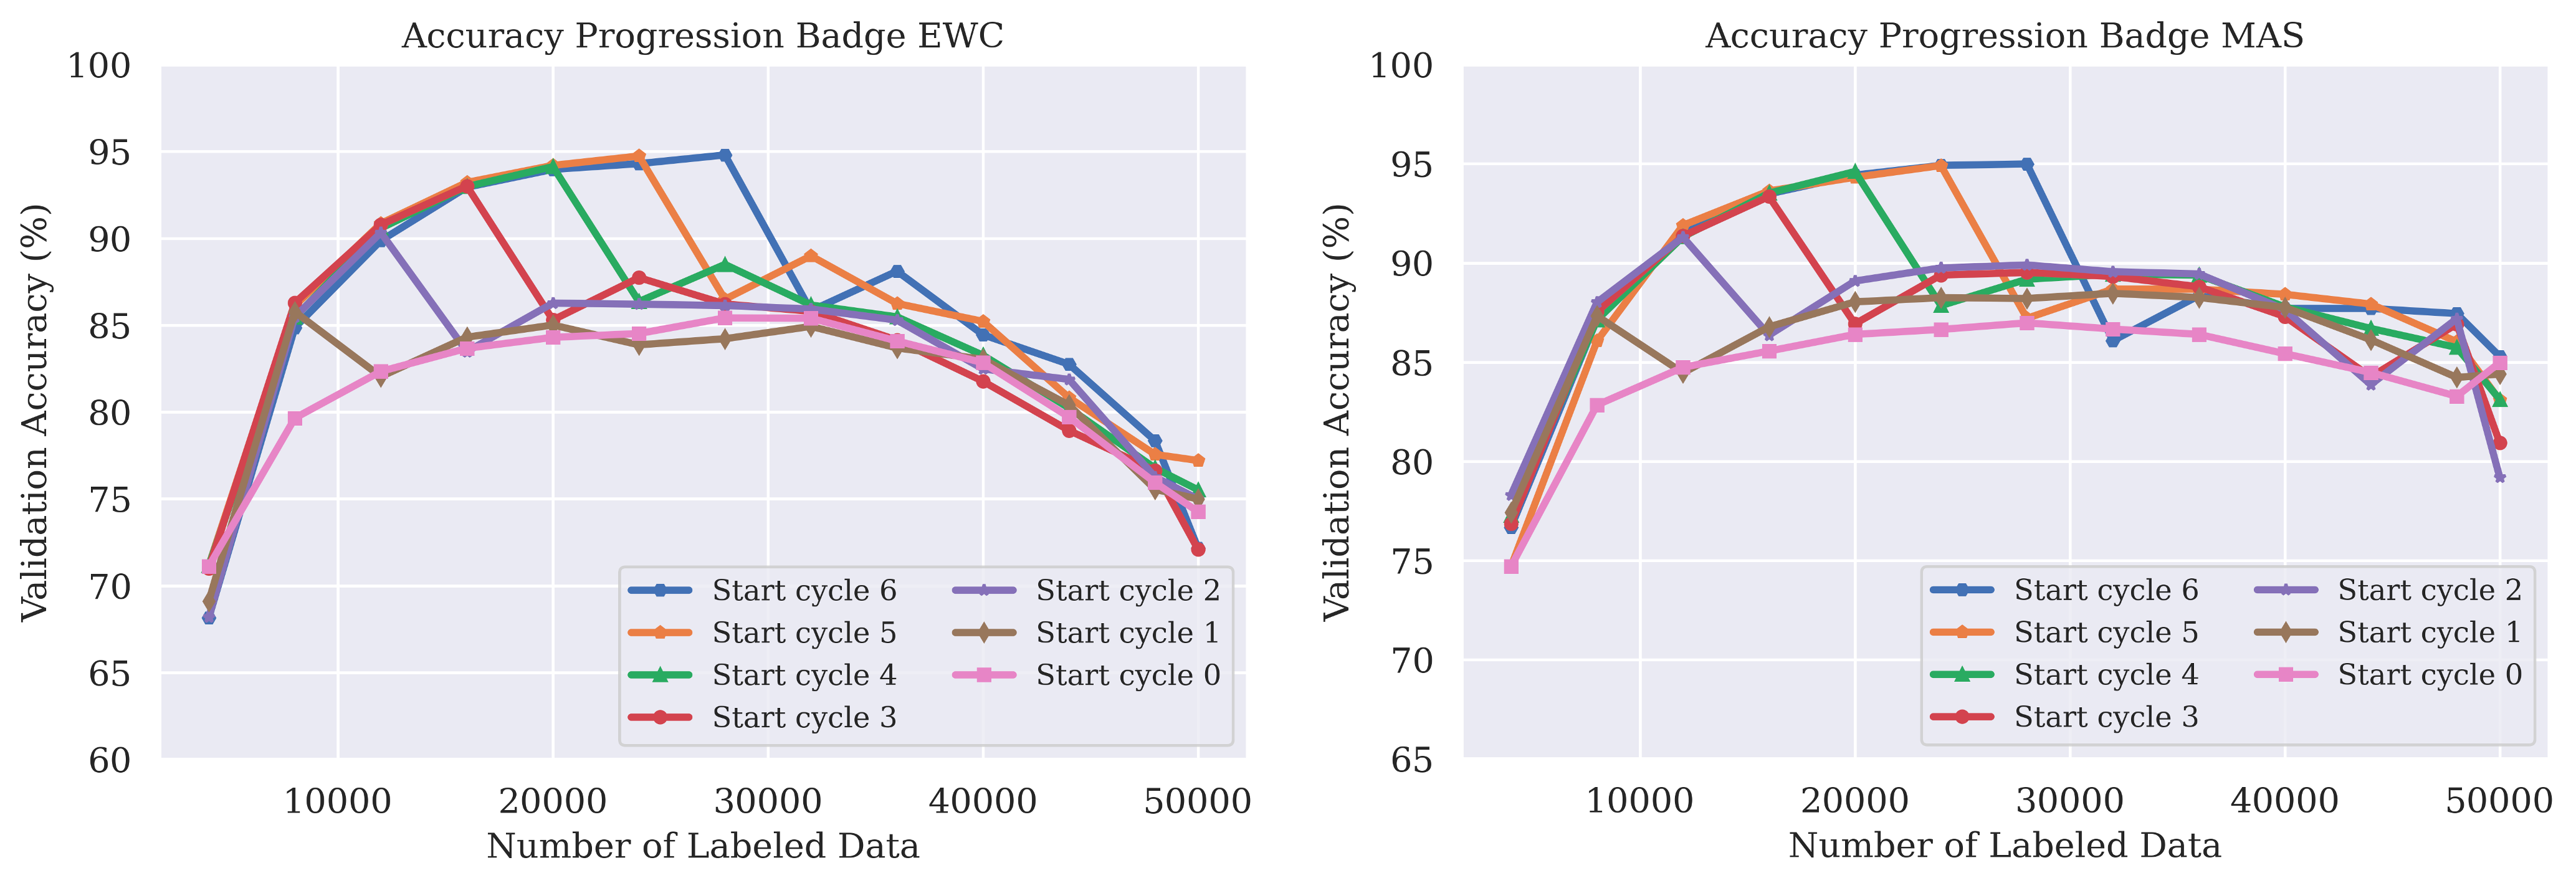
\includegraphics[width=\linewidth]{images/results_CAL/Delayed_start_CAL.png}
    \caption[Continual Active Learning Hybrid approach]{Comparison of validation accuracy for a delayed start of Continual Learning. }
    \label{fig:Evaluation:Results:CAL:DelayedStart}
\end{figure}

\subsubsection{Varying the initialization of the labeled pool}
\label{sec:Evaluation:Results:CAL:Initialization}
Motivated by the findings from the previous section, we wonder if the initialization of the labeled pool has an impact on the validation accuracy of the Continual Learning strategies. Beck et al.\cite{beck2021effective} show that using a facility location selection 
\cite{iyer2021submodular} yields better validation accuracy when training on the initial labeled pool. We therefore test the effect of an initialization using the facility location selection compared to our random initialization. As our Active Learning strategy,
we use Badge with a batch size of 4000 and MAS as our Continual Learning strategy. The results of the experiment can be found in figure \ref{fig:Evaluation:Results:CAL:FLinit}. While the facility location approach performs better than random initialization, the difference is
marginal. Interestingly, the validation accuracy of the facility location approach is lower than the random initialization in the first iteration. The most significant drawback of the facility location initialization is its resource-intensity. Initialization with facility
location takes about 24 hours to complete and requires more than 100GB of memory using the implementation proposed by Beck et al. \cite{beck2021effective}. \par

\begin{figure}[h]
    \centering
    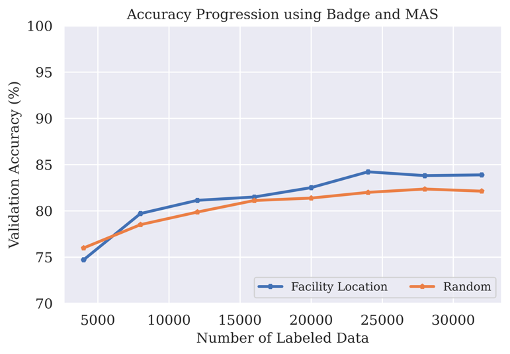
\includegraphics[width=\linewidth]{images/results_CAL/Factility_location_init.png}
    \caption[Initialization using Facility Location]{Comparison of validation accuracy for facility location initialization and random initialization. We use a batch size of 4000 for the experiments.}
    \label{fig:Evaluation:Results:CAL:FLinit}
\end{figure}


\subsubsection{Custom Replay approach}
\label{sec:Evaluation:Results:CAL:Replay}
In section \ref{sec:Methodology:ReplayStrategy} we propose a custom replay strategy for Continual Active Learning. The use of our replay strategy is motivated by the main finding of section \ref{sec:Evaluation:Results:CAL:ALCL}: the validation accuracy increases with an
increased batch size. In this set of experiments, we use the Active Learning strategy CoreSet and vary the batch size and the size of the replay buffer. Moreover, we investigate the effect of CoreSet selection in the replay buffer compared to random selection. We present our
results in figure \ref{fig:Evaluation:Results:CAL:Replay}. When variying the batch size and buffer size,  we notice 

\begin{figure}[h]
    \centering
    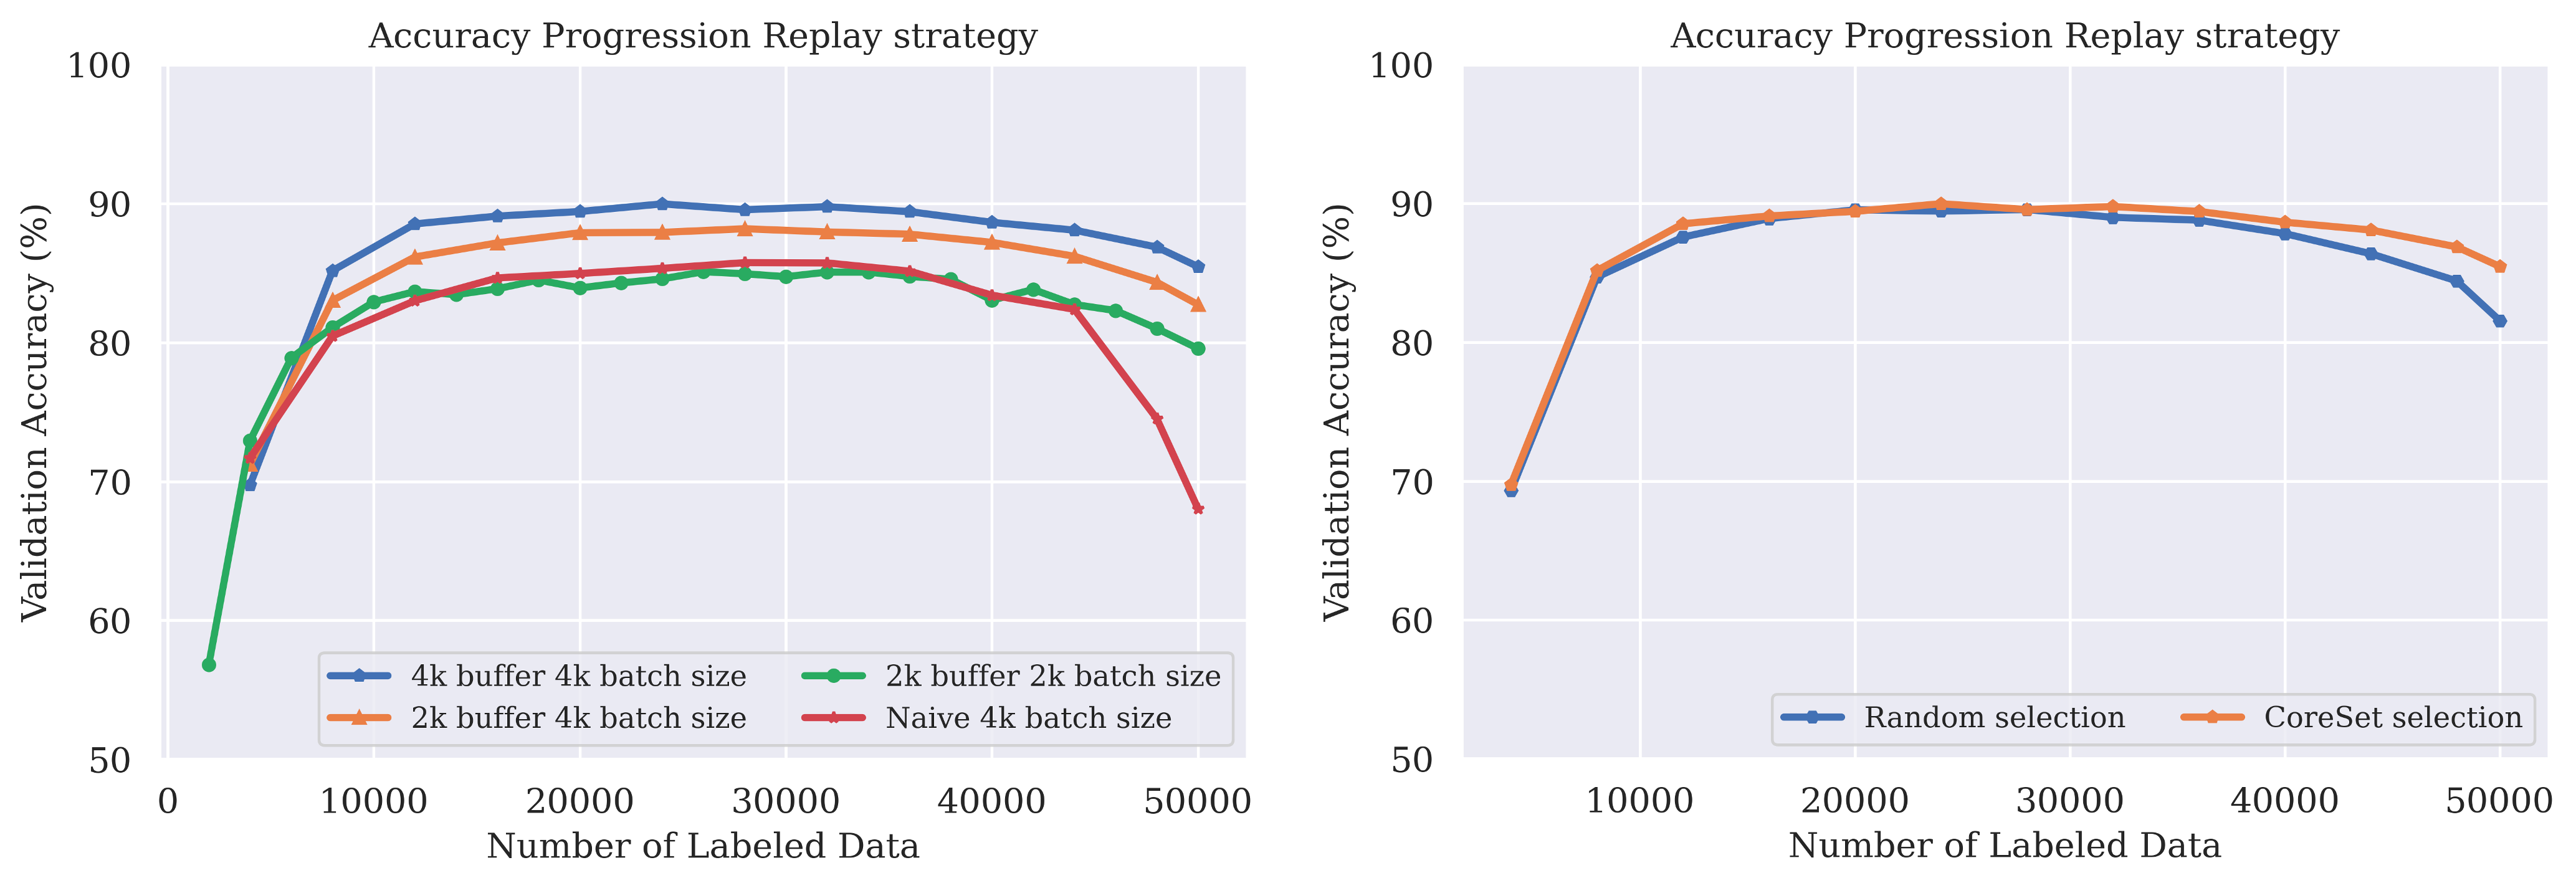
\includegraphics[width=\linewidth]{images/results_CAL/replay_CAL.png}
    \caption[Continual Active Learning Custom Replay strategy]{TODO: Redo plot}
    \label{fig:Evaluation:Results:CAL:Replay}
\end{figure}

\subsection{Results for Continual Active Learning for Model Stealing}
\label{sec:Evaluation:Results:CALMS}

\begin{table}
    \centering
    \begin{tabularx}{\textwidth}{l | c c c} 
        \hline
        \diaghead{\theadfont Diag ColumnHead 2}%
        {Target \\ Model}{Substitute \\ Model} &  ActiveThiefConv2 & ActiveThiefConv3 & ActiveThiefConv4 \\ 
        \hline 
        ActiveThiefConv2 & A & B & C \\
        ActiveThiefConv3 & A & B & C \\
        ActiveThiefConv4 & A & B & C \\
        \hline
    \end{tabularx}
    \caption{Success of Model Stealing Attacks for Different NN Architectures on CIFAR-10}
    \label{fig:ModelStealingNNArchitecturesCIFAR}
\end{table}


\begin{table}
    \centering
    \begin{tabularx}{\textwidth}{l | c c c} 
        \hline
        \diaghead{\theadfont Diag ColumnHead 2}%
        {Target \\ Model}{Substitute \\ Model} &  ActiveThiefConv2 & ActiveThiefConv3 & ActiveThiefConv4 \\ 
        \hline 
        ActiveThiefConv2 & A & B & C \\
        ActiveThiefConv3 & A & B & C \\
        ActiveThiefConv4 & A & B & C \\
        \hline
    \end{tabularx}
    \caption{Success of Model Stealing Attacks for Different NN Architectures on MNIST}
    \label{fig:ModelStealingNNArchitecturesMNIST}
\end{table}

\section{Discussion}
\label{sec:Evaluation:ThirdSection}
% Was war das Ziel? Was wurde (nicht) erreicht?

\dots
%% ---------------------
%% | / Example content |
%% ---------------------